\documentclass[twoside]{book}

% Packages required by doxygen
\usepackage{calc}
\usepackage{doxygen}
\usepackage{graphicx}
\usepackage[utf8]{inputenc}
\usepackage{makeidx}
\usepackage{multicol}
\usepackage{multirow}
\usepackage{textcomp}
\usepackage[table]{xcolor}

% Font selection
\usepackage[T1]{fontenc}
\usepackage{mathptmx}
\usepackage[scaled=.90]{helvet}
\usepackage{courier}
\usepackage{amssymb}
\usepackage{sectsty}
\renewcommand{\familydefault}{\sfdefault}
\allsectionsfont{%
  \fontseries{bc}\selectfont%
  \color{darkgray}%
}
\renewcommand{\DoxyLabelFont}{%
  \fontseries{bc}\selectfont%
  \color{darkgray}%
}

% Page & text layout
\usepackage{geometry}
\geometry{%
  a4paper,%
  top=2.5cm,%
  bottom=2.5cm,%
  left=2.5cm,%
  right=2.5cm%
}
\tolerance=750
\hfuzz=15pt
\hbadness=750
\setlength{\emergencystretch}{15pt}
\setlength{\parindent}{0cm}
\setlength{\parskip}{0.2cm}
\makeatletter
\renewcommand{\paragraph}{%
  \@startsection{paragraph}{4}{0ex}{-1.0ex}{1.0ex}{%
    \normalfont\normalsize\bfseries\SS@parafont%
  }%
}
\renewcommand{\subparagraph}{%
  \@startsection{subparagraph}{5}{0ex}{-1.0ex}{1.0ex}{%
    \normalfont\normalsize\bfseries\SS@subparafont%
  }%
}
\makeatother

% Headers & footers
\usepackage{fancyhdr}
\pagestyle{fancyplain}
\fancyhead[LE]{\fancyplain{}{\bfseries\thepage}}
\fancyhead[CE]{\fancyplain{}{}}
\fancyhead[RE]{\fancyplain{}{\bfseries\leftmark}}
\fancyhead[LO]{\fancyplain{}{\bfseries\rightmark}}
\fancyhead[CO]{\fancyplain{}{}}
\fancyhead[RO]{\fancyplain{}{\bfseries\thepage}}
\fancyfoot[LE]{\fancyplain{}{}}
\fancyfoot[CE]{\fancyplain{}{}}
\fancyfoot[RE]{\fancyplain{}{\bfseries\scriptsize Generated on Sat May 3 2014 20\-:23\-:19 for Bad Philophobia by Doxygen }}
\fancyfoot[LO]{\fancyplain{}{\bfseries\scriptsize Generated on Sat May 3 2014 20\-:23\-:19 for Bad Philophobia by Doxygen }}
\fancyfoot[CO]{\fancyplain{}{}}
\fancyfoot[RO]{\fancyplain{}{}}
\renewcommand{\footrulewidth}{0.4pt}
\renewcommand{\chaptermark}[1]{%
  \markboth{#1}{}%
}
\renewcommand{\sectionmark}[1]{%
  \markright{\thesection\ #1}%
}

% Indices & bibliography
\usepackage{natbib}
\usepackage[titles]{tocloft}
\setcounter{tocdepth}{3}
\setcounter{secnumdepth}{5}
\makeindex

% Hyperlinks (required, but should be loaded last)
\usepackage{ifpdf}
\ifpdf
  \usepackage[pdftex,pagebackref=true]{hyperref}
\else
  \usepackage[ps2pdf,pagebackref=true]{hyperref}
\fi
\hypersetup{%
  colorlinks=true,%
  linkcolor=blue,%
  citecolor=blue,%
  unicode%
}

% Custom commands
\newcommand{\clearemptydoublepage}{%
  \newpage{\pagestyle{empty}\cleardoublepage}%
}


%===== C O N T E N T S =====

\begin{document}

% Titlepage & ToC
\hypersetup{pageanchor=false}
\pagenumbering{roman}
\begin{titlepage}
\vspace*{7cm}
\begin{center}%
{\Large Bad Philophobia }\\
\vspace*{1cm}
{\large Generated by Doxygen 1.8.6}\\
\vspace*{0.5cm}
{\small Sat May 3 2014 20:23:19}\\
\end{center}
\end{titlepage}
\clearemptydoublepage
\tableofcontents
\clearemptydoublepage
\pagenumbering{arabic}
\hypersetup{pageanchor=true}

%--- Begin generated contents ---
\chapter{Hierarchical Index}
\section{Class Hierarchy}
This inheritance list is sorted roughly, but not completely, alphabetically\-:\begin{DoxyCompactList}
\item Action\-Listener\begin{DoxyCompactList}
\item \contentsline{section}{User\-Interface}{\pageref{classUserInterface}}{}
\end{DoxyCompactList}
\item \contentsline{section}{Command\-Words}{\pageref{classCommandWords}}{}
\item \contentsline{section}{Game}{\pageref{classGame}}{}
\item \contentsline{section}{Game\-Engine}{\pageref{classGameEngine}}{}
\item \contentsline{section}{Parser}{\pageref{classParser}}{}
\item \contentsline{section}{Room}{\pageref{classRoom}}{}
\end{DoxyCompactList}

\chapter{Class Index}
\section{Class List}
Here are the classes, structs, unions and interfaces with brief descriptions\-:\begin{DoxyCompactList}
\item\contentsline{section}{\hyperlink{classCommandWords}{Command\-Words} }{\pageref{classCommandWords}}{}
\item\contentsline{section}{\hyperlink{classGame}{Game} }{\pageref{classGame}}{}
\item\contentsline{section}{\hyperlink{classGameEngine}{Game\-Engine} }{\pageref{classGameEngine}}{}
\item\contentsline{section}{\hyperlink{classParser}{Parser} }{\pageref{classParser}}{}
\item\contentsline{section}{\hyperlink{classRoom}{Room} }{\pageref{classRoom}}{}
\item\contentsline{section}{\hyperlink{classUserInterface}{User\-Interface} }{\pageref{classUserInterface}}{}
\end{DoxyCompactList}

\chapter{File Index}
\section{File List}
Here is a list of all files with brief descriptions\-:\begin{DoxyCompactList}
\item\contentsline{section}{\hyperlink{Command_8java}{Command.\-java} }{\pageref{Command_8java}}{}
\item\contentsline{section}{\hyperlink{CommandWords_8java}{Command\-Words.\-java} }{\pageref{CommandWords_8java}}{}
\item\contentsline{section}{\hyperlink{Game_8java}{Game.\-java} }{\pageref{Game_8java}}{}
\item\contentsline{section}{\hyperlink{GameEngine_8java}{Game\-Engine.\-java} }{\pageref{GameEngine_8java}}{}
\item\contentsline{section}{\hyperlink{Item_8java}{Item.\-java} }{\pageref{Item_8java}}{}
\item\contentsline{section}{\hyperlink{Parser_8java}{Parser.\-java} }{\pageref{Parser_8java}}{}
\item\contentsline{section}{\hyperlink{Room_8java}{Room.\-java} }{\pageref{Room_8java}}{}
\item\contentsline{section}{\hyperlink{UserInterface_8java}{User\-Interface.\-java} }{\pageref{UserInterface_8java}}{}
\end{DoxyCompactList}

\chapter{Class Documentation}
\hypertarget{classCommandWords}{\section{Command\-Words Class Reference}
\label{classCommandWords}\index{Command\-Words@{Command\-Words}}
}


Class used to verify the commands given by the user.  




Collaboration diagram for Command\-Words\-:
\nopagebreak
\begin{figure}[H]
\begin{center}
\leavevmode
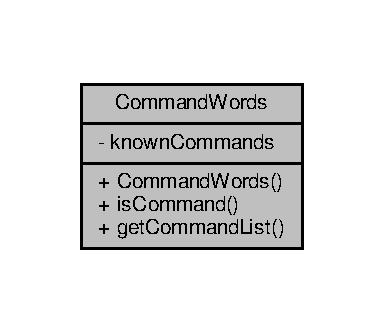
\includegraphics[width=232pt]{classCommandWords__coll__graph}
\end{center}
\end{figure}
\subsection*{Public Member Functions}
\begin{DoxyCompactItemize}
\item 
\hyperlink{classCommandWords_a2d8c096723adb3f822cc001bccd92ed7}{Command\-Words} ()
\begin{DoxyCompactList}\small\item\em \hyperlink{classCommandWords}{Command\-Words} class constructor. \end{DoxyCompactList}\item 
boolean \hyperlink{classCommandWords_a646ed94a6d8d190b7cc445378ee2306e}{is\-Command} (String command)
\begin{DoxyCompactList}\small\item\em Check if the command is known. \end{DoxyCompactList}\item 
String \hyperlink{classCommandWords_aa26f54985e39543739e0ae291dcdb8f1}{get\-Command\-List} ()
\begin{DoxyCompactList}\small\item\em Getter for the known\-Commands field. \end{DoxyCompactList}\item 
\hyperlink{classCommand}{Command} \hyperlink{classCommandWords_af89bc564e4cf32021721ca44f46de6cb}{get\-Command} (String command\-Word)
\begin{DoxyCompactList}\small\item\em Find the \hyperlink{enumCommandWord}{Command\-Word} associated with a command word. \end{DoxyCompactList}\end{DoxyCompactItemize}
\subsection*{Private Attributes}
\begin{DoxyCompactItemize}
\item 
Hash\-Map$<$ String, \hyperlink{classCommand}{Command} $>$ \hyperlink{classCommandWords_a87d12c01410f3c523f7889d523d537e7}{commands}
\end{DoxyCompactItemize}


\subsection{Detailed Description}
Class used to verify the commands given by the user. 

It contains all known commands and can verify if a String is a known command. \begin{DoxyAuthor}{Author}
Rémi N\-I\-C\-O\-L\-E 
\end{DoxyAuthor}


Definition at line \hyperlink{CommandWords_8java_source_l00011}{11} of file \hyperlink{CommandWords_8java_source}{Command\-Words.\-java}.



\subsection{Constructor \& Destructor Documentation}
\hypertarget{classCommandWords_a2d8c096723adb3f822cc001bccd92ed7}{\index{Command\-Words@{Command\-Words}!Command\-Words@{Command\-Words}}
\index{Command\-Words@{Command\-Words}!CommandWords@{Command\-Words}}
\subsubsection[{Command\-Words}]{\setlength{\rightskip}{0pt plus 5cm}Command\-Words.\-Command\-Words (
\begin{DoxyParamCaption}
{}
\end{DoxyParamCaption}
)}}\label{classCommandWords_a2d8c096723adb3f822cc001bccd92ed7}


\hyperlink{classCommandWords}{Command\-Words} class constructor. 



Definition at line \hyperlink{CommandWords_8java_source_l00018}{18} of file \hyperlink{CommandWords_8java_source}{Command\-Words.\-java}.



References \hyperlink{CommandWords_8java_source_l00013}{commands}.


\begin{DoxyCode}
00018                           \{
00019         \hyperlink{classCommandWords_a87d12c01410f3c523f7889d523d537e7}{commands} = \textcolor{keyword}{new} HashMap<String, Command>();
00020         commands.put(\textcolor{stringliteral}{"go"}, \textcolor{keyword}{new} \hyperlink{classGoCommand}{GoCommand}());
00021         commands.put(\textcolor{stringliteral}{"back"}, \textcolor{keyword}{new} \hyperlink{classBackCommand}{BackCommand}());
00022         commands.put(\textcolor{stringliteral}{"beamer"}, \textcolor{keyword}{new} \hyperlink{classBeamerCommand}{BeamerCommand}());
00023         commands.put(\textcolor{stringliteral}{"look"}, \textcolor{keyword}{new} \hyperlink{classLookCommand}{LookCommand}());
00024         commands.put(\textcolor{stringliteral}{"take"}, \textcolor{keyword}{new} \hyperlink{classTakeCommand}{TakeCommand}());
00025         commands.put(\textcolor{stringliteral}{"drop"}, \textcolor{keyword}{new} \hyperlink{classDropCommand}{DropCommand}());
00026         commands.put(\textcolor{stringliteral}{"inventory"}, \textcolor{keyword}{new} \hyperlink{classInventoryCommand}{InventoryCommand}());
00027         commands.put(\textcolor{stringliteral}{"eat"}, \textcolor{keyword}{new} \hyperlink{classEatCommand}{EatCommand}());
00028         commands.put(\textcolor{stringliteral}{"test"}, \textcolor{keyword}{new} \hyperlink{classTestCommand}{TestCommand}());
00029         commands.put(\textcolor{stringliteral}{"quit"}, \textcolor{keyword}{new} \hyperlink{classQuitCommand}{QuitCommand}());
00030         commands.put(\textcolor{stringliteral}{"help"}, \textcolor{keyword}{new} \hyperlink{classHelpCommand}{HelpCommand}());
00031         commands.put(\textcolor{stringliteral}{"credits"}, \textcolor{keyword}{new} \hyperlink{classCreditsCommand}{CreditsCommand}());
00032     \}
\end{DoxyCode}


\subsection{Member Function Documentation}
\hypertarget{classCommandWords_af89bc564e4cf32021721ca44f46de6cb}{\index{Command\-Words@{Command\-Words}!get\-Command@{get\-Command}}
\index{get\-Command@{get\-Command}!CommandWords@{Command\-Words}}
\subsubsection[{get\-Command}]{\setlength{\rightskip}{0pt plus 5cm}{\bf Command} Command\-Words.\-get\-Command (
\begin{DoxyParamCaption}
\item[{String}]{command\-Word}
\end{DoxyParamCaption}
)}}\label{classCommandWords_af89bc564e4cf32021721ca44f46de6cb}


Find the \hyperlink{enumCommandWord}{Command\-Word} associated with a command word. 


\begin{DoxyParams}{Parameters}
{\em command\-Word} & The word to look up. \\
\hline
\end{DoxyParams}
\begin{DoxyReturn}{Returns}
The \hyperlink{classCommand}{Command} correspondng to command\-Word, or null if it is not a valid command word. 
\end{DoxyReturn}


Definition at line \hyperlink{CommandWords_8java_source_l00062}{62} of file \hyperlink{CommandWords_8java_source}{Command\-Words.\-java}.


\begin{DoxyCode}
00063     \{
00064         \textcolor{keywordflow}{return} commands.get(commandWord);
00065     \}
\end{DoxyCode}
\hypertarget{classCommandWords_aa26f54985e39543739e0ae291dcdb8f1}{\index{Command\-Words@{Command\-Words}!get\-Command\-List@{get\-Command\-List}}
\index{get\-Command\-List@{get\-Command\-List}!CommandWords@{Command\-Words}}
\subsubsection[{get\-Command\-List}]{\setlength{\rightskip}{0pt plus 5cm}String Command\-Words.\-get\-Command\-List (
\begin{DoxyParamCaption}
{}
\end{DoxyParamCaption}
)}}\label{classCommandWords_aa26f54985e39543739e0ae291dcdb8f1}


Getter for the known\-Commands field. 

\begin{DoxyReturn}{Returns}
The list of available commands 
\end{DoxyReturn}


Definition at line \hyperlink{CommandWords_8java_source_l00047}{47} of file \hyperlink{CommandWords_8java_source}{Command\-Words.\-java}.


\begin{DoxyCode}
00047                                    \{
00048         String commandsString = \textcolor{stringliteral}{""};
00049         Iterator<String> it = commands.keySet().iterator();
00050         \textcolor{keywordflow}{while}(it.hasNext()) \{
00051             String command = it.next();
00052             commandsString += command + ((it.hasNext())? \textcolor{stringliteral}{", "} : \textcolor{stringliteral}{"."});
00053         \}
00054         \textcolor{keywordflow}{return} commandsString;
00055     \}
\end{DoxyCode}
\hypertarget{classCommandWords_a646ed94a6d8d190b7cc445378ee2306e}{\index{Command\-Words@{Command\-Words}!is\-Command@{is\-Command}}
\index{is\-Command@{is\-Command}!CommandWords@{Command\-Words}}
\subsubsection[{is\-Command}]{\setlength{\rightskip}{0pt plus 5cm}boolean Command\-Words.\-is\-Command (
\begin{DoxyParamCaption}
\item[{String}]{command}
\end{DoxyParamCaption}
)}}\label{classCommandWords_a646ed94a6d8d190b7cc445378ee2306e}


Check if the command is known. 


\begin{DoxyParams}{Parameters}
{\em command} & The command to check \\
\hline
\end{DoxyParams}
\begin{DoxyReturn}{Returns}
True if and only if the command is known. 
\end{DoxyReturn}


Definition at line \hyperlink{CommandWords_8java_source_l00039}{39} of file \hyperlink{CommandWords_8java_source}{Command\-Words.\-java}.


\begin{DoxyCode}
00039                                              \{
00040         \textcolor{keywordflow}{return} commands.containsKey(command);
00041     \}
\end{DoxyCode}


\subsection{Member Data Documentation}
\hypertarget{classCommandWords_a87d12c01410f3c523f7889d523d537e7}{\index{Command\-Words@{Command\-Words}!commands@{commands}}
\index{commands@{commands}!CommandWords@{Command\-Words}}
\subsubsection[{commands}]{\setlength{\rightskip}{0pt plus 5cm}Hash\-Map$<$String, {\bf Command}$>$ Command\-Words.\-commands\hspace{0.3cm}{\ttfamily [private]}}}\label{classCommandWords_a87d12c01410f3c523f7889d523d537e7}


Definition at line \hyperlink{CommandWords_8java_source_l00013}{13} of file \hyperlink{CommandWords_8java_source}{Command\-Words.\-java}.



Referenced by \hyperlink{CommandWords_8java_source_l00018}{Command\-Words()}.



The documentation for this class was generated from the following file\-:\begin{DoxyCompactItemize}
\item 
\hyperlink{CommandWords_8java}{Command\-Words.\-java}\end{DoxyCompactItemize}

\hypertarget{classGame}{\section{Game Class Reference}
\label{classGame}\index{Game@{Game}}
}


Main class used to instantiate other objects.  




Collaboration diagram for Game\-:
\nopagebreak
\begin{figure}[H]
\begin{center}
\leavevmode
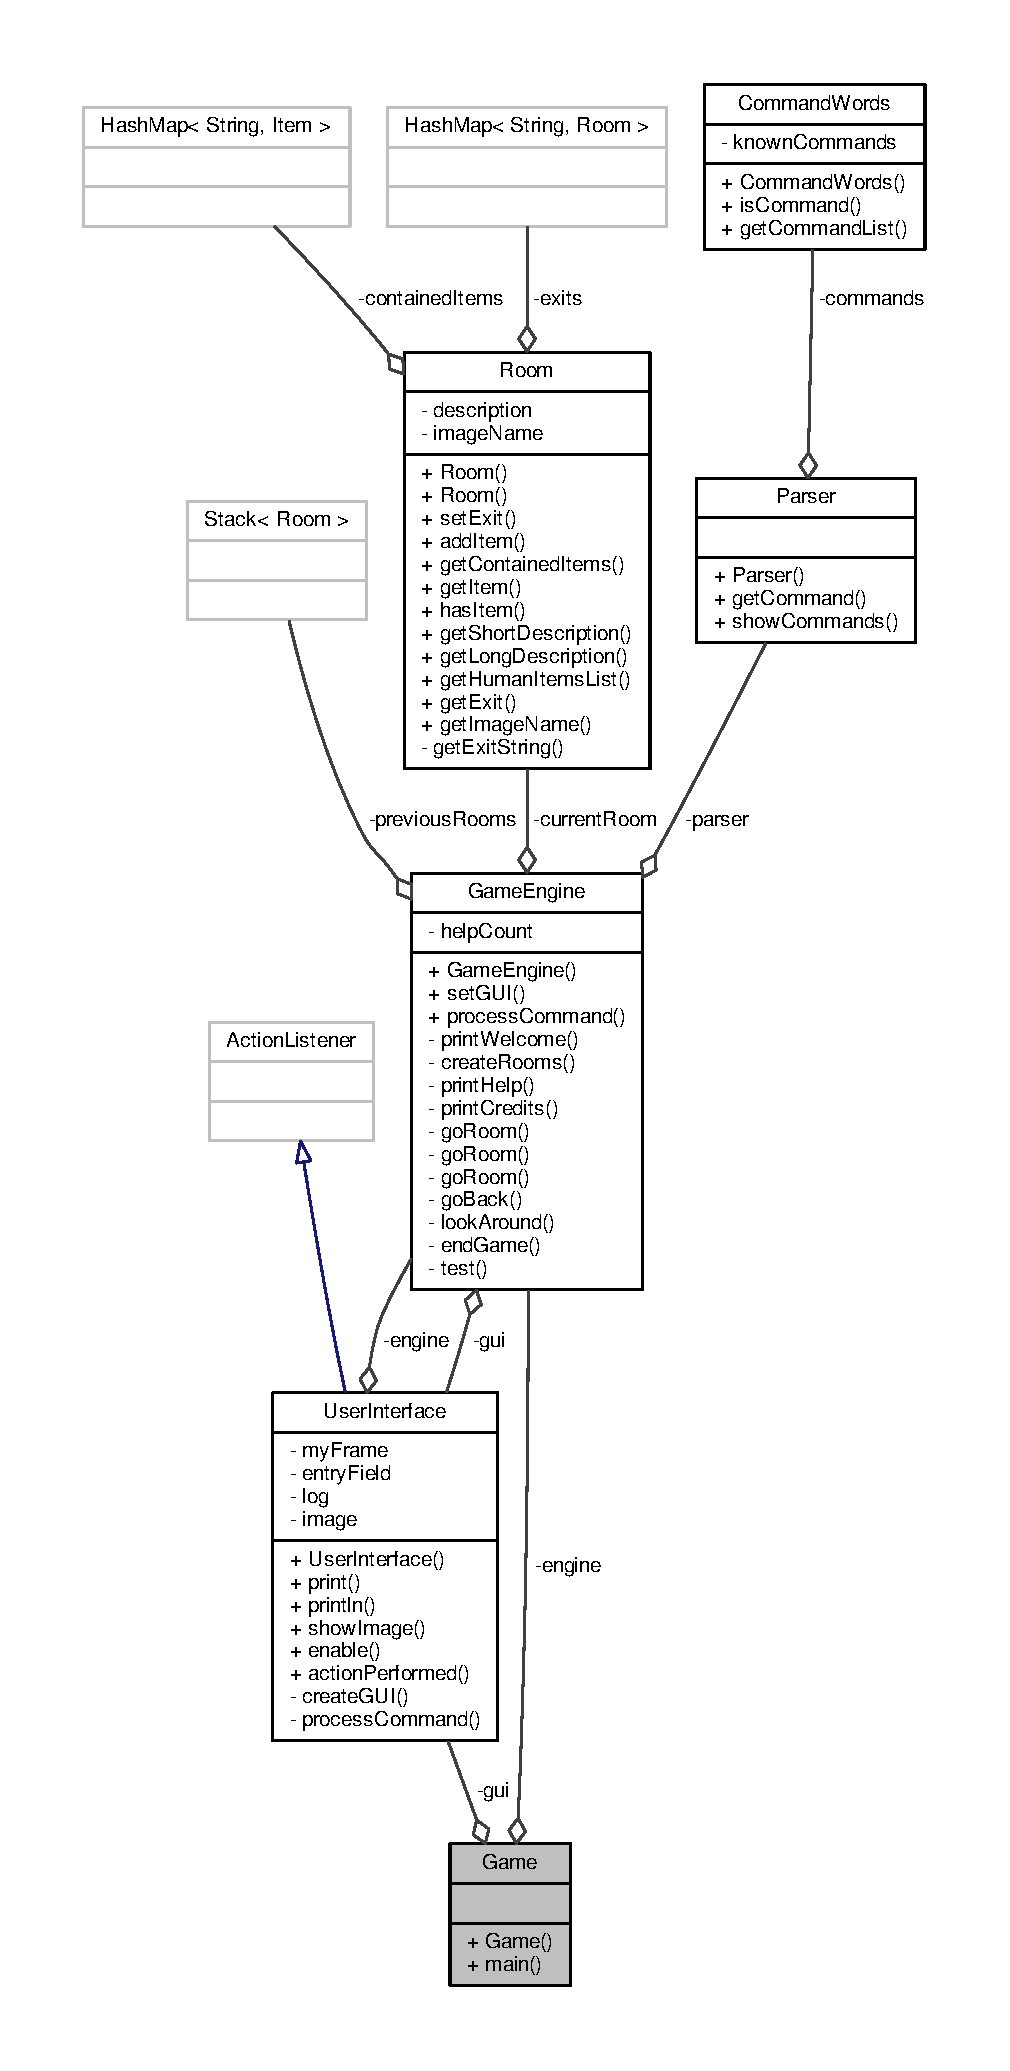
\includegraphics[width=136pt]{classGame__coll__graph}
\end{center}
\end{figure}
\subsection*{Public Member Functions}
\begin{DoxyCompactItemize}
\item 
\hyperlink{classGame_a2e034e53e9c032964ecd2a831b29a616}{Game} ()
\begin{DoxyCompactList}\small\item\em \hyperlink{classGame}{Game} class constructor. \end{DoxyCompactList}\end{DoxyCompactItemize}
\subsection*{Static Public Member Functions}
\begin{DoxyCompactItemize}
\item 
static void \hyperlink{classGame_ae52595a27ac1b327b05db2129ad81fca}{main} (String\mbox{[}$\,$\mbox{]} args)
\begin{DoxyCompactList}\small\item\em Main function. \end{DoxyCompactList}\end{DoxyCompactItemize}


\subsection{Detailed Description}
Main class used to instantiate other objects. 

\begin{DoxyAuthor}{Author}
Rémi N\-I\-C\-O\-L\-E 
\end{DoxyAuthor}


Definition at line \hyperlink{Game_8java_source_l00009}{9} of file \hyperlink{Game_8java_source}{Game.\-java}.



\subsection{Constructor \& Destructor Documentation}
\hypertarget{classGame_a2e034e53e9c032964ecd2a831b29a616}{\index{Game@{Game}!Game@{Game}}
\index{Game@{Game}!Game@{Game}}
\subsubsection[{Game}]{\setlength{\rightskip}{0pt plus 5cm}Game.\-Game (
\begin{DoxyParamCaption}
{}
\end{DoxyParamCaption}
)}}\label{classGame_a2e034e53e9c032964ecd2a831b29a616}


\hyperlink{classGame}{Game} class constructor. 



Definition at line \hyperlink{Game_8java_source_l00032}{32} of file \hyperlink{Game_8java_source}{Game.\-java}.



Referenced by \hyperlink{Game_8java_source_l00015}{main()}.


\begin{DoxyCode}
00032                    \{
00033         engine = \textcolor{keyword}{new} \hyperlink{classpkg__game_1_1GameEngine}{GameEngine}();
00034         gui = \textcolor{keyword}{new} \hyperlink{classpkg__game_1_1UserInterface}{UserInterface}(engine);
00035         engine.setGUI(gui);
00036     \}
\end{DoxyCode}


Here is the caller graph for this function\-:
\nopagebreak
\begin{figure}[H]
\begin{center}
\leavevmode
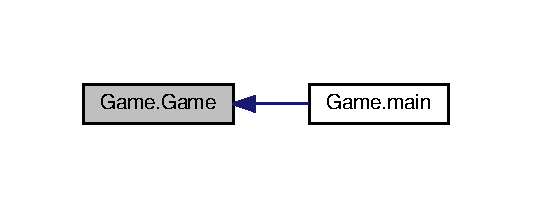
\includegraphics[width=256pt]{classGame_a2e034e53e9c032964ecd2a831b29a616_icgraph}
\end{center}
\end{figure}




\subsection{Member Function Documentation}
\hypertarget{classGame_ae52595a27ac1b327b05db2129ad81fca}{\index{Game@{Game}!main@{main}}
\index{main@{main}!Game@{Game}}
\subsubsection[{main}]{\setlength{\rightskip}{0pt plus 5cm}static void Game.\-main (
\begin{DoxyParamCaption}
\item[{String\mbox{[}$\,$\mbox{]}}]{args}
\end{DoxyParamCaption}
)\hspace{0.3cm}{\ttfamily [static]}}}\label{classGame_ae52595a27ac1b327b05db2129ad81fca}


Main function. 


\begin{DoxyParams}{Parameters}
{\em args} & Command line arguments \\
\hline
\end{DoxyParams}


Definition at line \hyperlink{Game_8java_source_l00015}{15} of file \hyperlink{Game_8java_source}{Game.\-java}.



References \hyperlink{Game_8java_source_l00032}{Game()}.


\begin{DoxyCode}
00015                                            \{
00016         \hyperlink{classGame}{Game} game = \textcolor{keyword}{new} \hyperlink{classGame_a2e034e53e9c032964ecd2a831b29a616}{Game}();
00017     \}
\end{DoxyCode}


Here is the call graph for this function\-:
\nopagebreak
\begin{figure}[H]
\begin{center}
\leavevmode
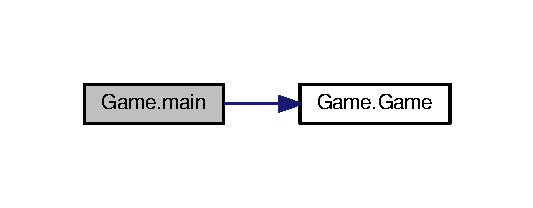
\includegraphics[width=256pt]{classGame_ae52595a27ac1b327b05db2129ad81fca_cgraph}
\end{center}
\end{figure}




The documentation for this class was generated from the following file\-:\begin{DoxyCompactItemize}
\item 
\hyperlink{Game_8java}{Game.\-java}\end{DoxyCompactItemize}

\hypertarget{classGameEngine}{\section{Game\-Engine Class Reference}
\label{classGameEngine}\index{Game\-Engine@{Game\-Engine}}
}


Class handling the gameplay for the game.  




Collaboration diagram for Game\-Engine\-:
\nopagebreak
\begin{figure}[H]
\begin{center}
\leavevmode
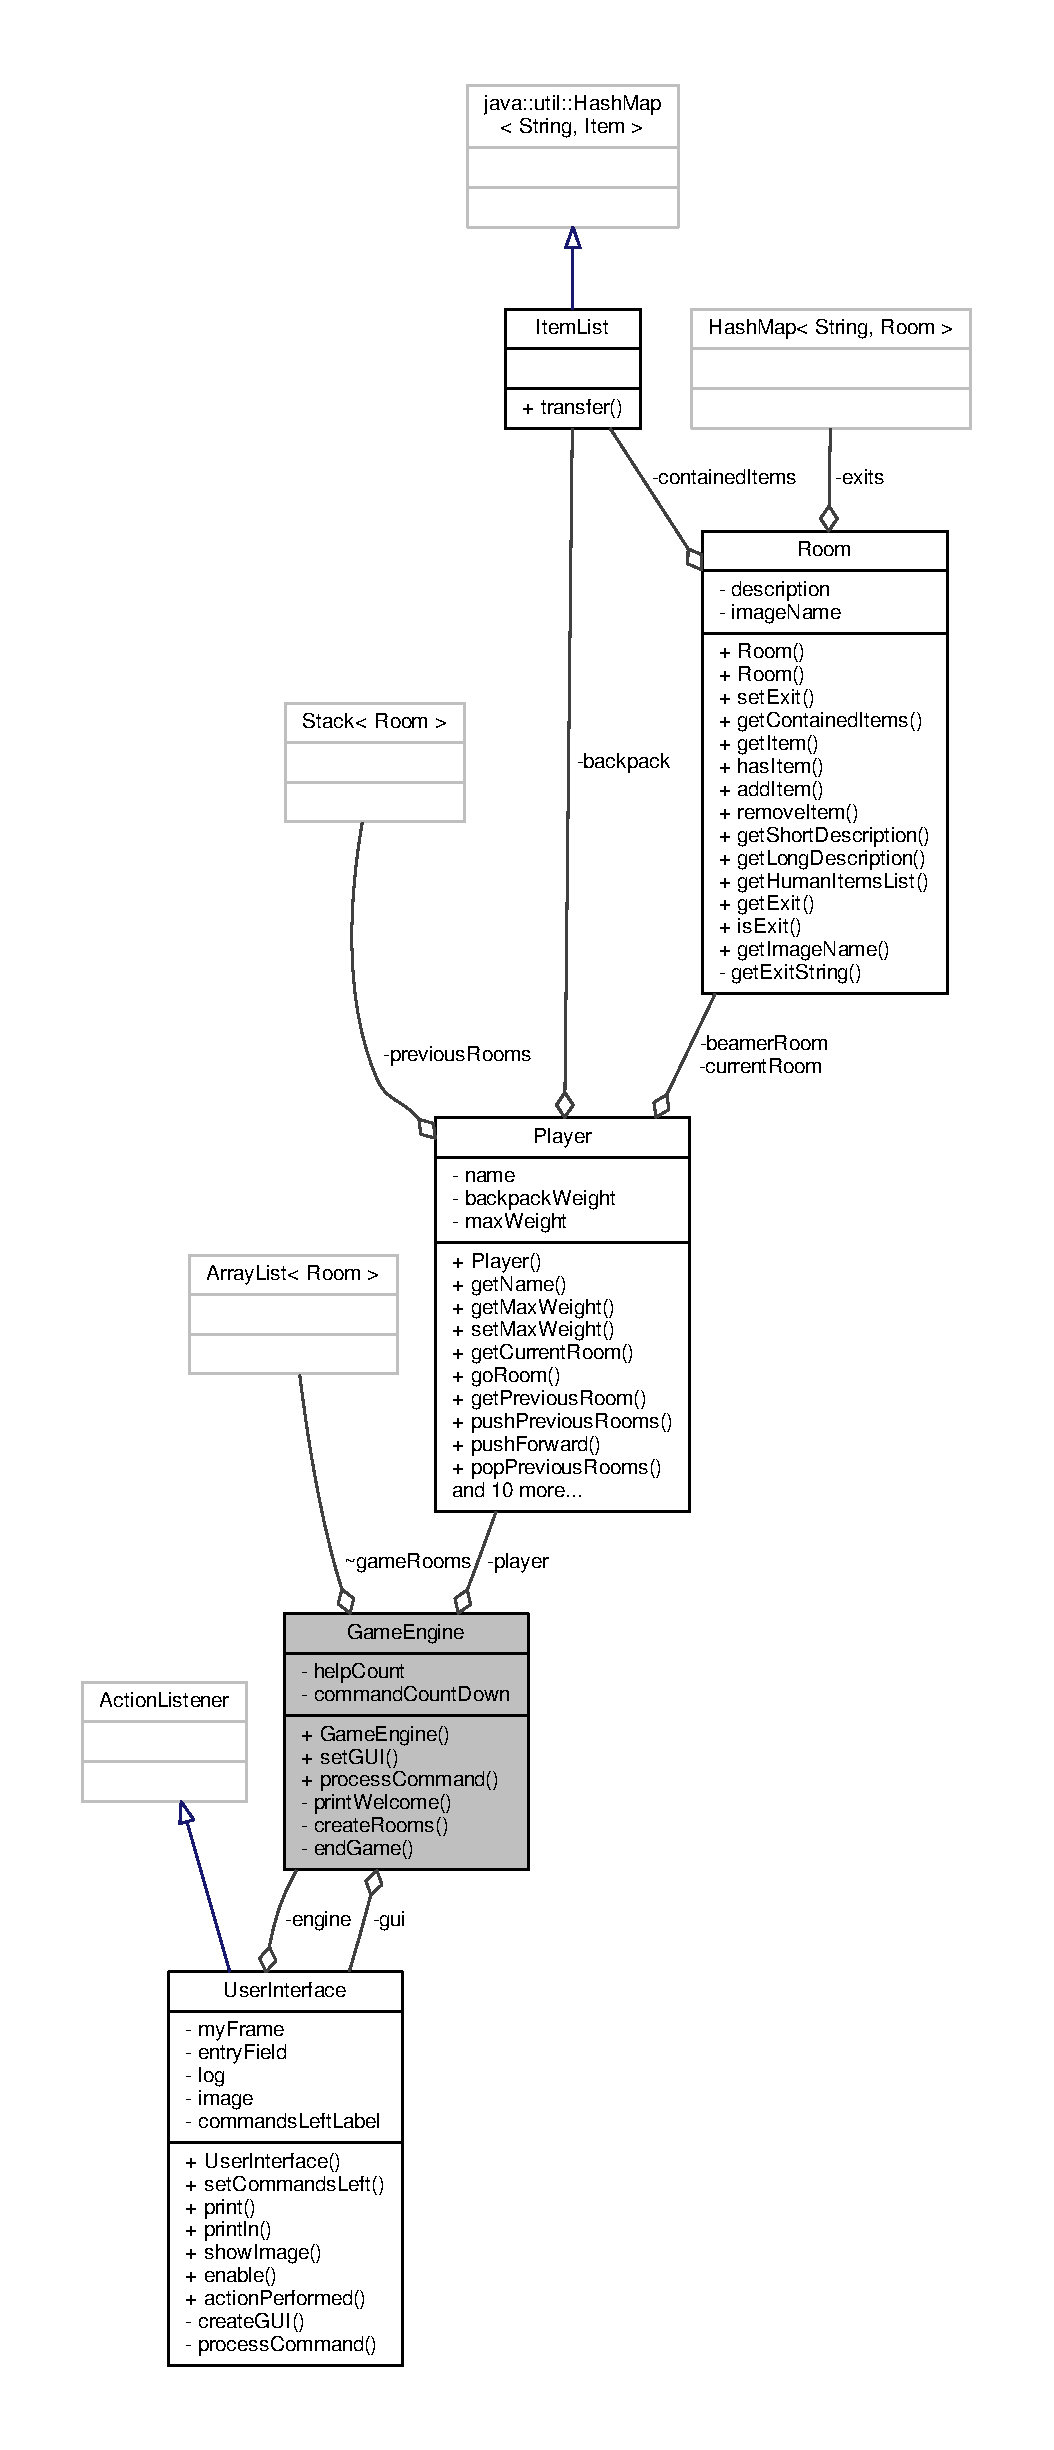
\includegraphics[height=550pt]{classGameEngine__coll__graph}
\end{center}
\end{figure}
\subsection*{Public Member Functions}
\begin{DoxyCompactItemize}
\item 
\hyperlink{classGameEngine_a9e8a92f5021a34293060f9aaff4005de}{Game\-Engine} ()
\begin{DoxyCompactList}\small\item\em \hyperlink{classGameEngine}{Game\-Engine} class constructor. \end{DoxyCompactList}\item 
void \hyperlink{classGameEngine_aec901a5b590b3cd204f196165da5dfb6}{set\-G\-U\-I} (\hyperlink{classUserInterface}{User\-Interface} user\-Interface)
\begin{DoxyCompactList}\small\item\em Setter for the gui field. \end{DoxyCompactList}\item 
void \hyperlink{classGameEngine_ad7133885f313fa99bca3bb7cb8272f64}{process\-Command} (String command\-Line)
\begin{DoxyCompactList}\small\item\em Process the command. \end{DoxyCompactList}\end{DoxyCompactItemize}
\subsection*{Package Attributes}
\begin{DoxyCompactItemize}
\item 
Array\-List$<$ \hyperlink{classRoom}{Room} $>$ \hyperlink{classGameEngine_ae5a2f252ec103e0630aebb8635341ea4}{game\-Rooms}
\begin{DoxyCompactList}\small\item\em A list of all the rooms in the game. \end{DoxyCompactList}\end{DoxyCompactItemize}
\subsection*{Private Member Functions}
\begin{DoxyCompactItemize}
\item 
void \hyperlink{classGameEngine_a9a2f3cb921bb19399e357bf14d26425b}{print\-Welcome} ()
\begin{DoxyCompactList}\small\item\em Welcome the user at the start of the game. \end{DoxyCompactList}\item 
\hyperlink{classRoom}{Room} \hyperlink{classGameEngine_a9410d92f7d0e6820059b1d07da364b09}{create\-Rooms} ()
\begin{DoxyCompactList}\small\item\em Create the rooms, link them and return the first \hyperlink{classRoom}{Room}. \end{DoxyCompactList}\item 
void \hyperlink{classGameEngine_a1f5fa36c5dfc36c9a963fe439afc057b}{end\-Game} (boolean winning)
\begin{DoxyCompactList}\small\item\em Print goodbye message and disable gui. \end{DoxyCompactList}\end{DoxyCompactItemize}
\subsection*{Private Attributes}
\begin{DoxyCompactItemize}
\item 
\hyperlink{classPlayer}{Player} \hyperlink{classGameEngine_a4666c6719428cc43014b30b305eeef5d}{player}
\begin{DoxyCompactList}\small\item\em \hyperlink{classPlayer}{Player} for the game. \end{DoxyCompactList}\item 
\hyperlink{classUserInterface}{User\-Interface} \hyperlink{classGameEngine_a2a7d0bb6183b3f3ef3ee2008926374a0}{gui}
\begin{DoxyCompactList}\small\item\em User interface for the game. \end{DoxyCompactList}\item 
int \hyperlink{classGameEngine_a308a9926d553d53cb4c56c28588f6c62}{help\-Count}
\begin{DoxyCompactList}\small\item\em Help query counter. \end{DoxyCompactList}\item 
int \hyperlink{classGameEngine_ad4ff8d760eced9c7b76cdeb0dc989975}{command\-Count\-Down}
\begin{DoxyCompactList}\small\item\em The command number limit of the game. \end{DoxyCompactList}\end{DoxyCompactItemize}


\subsection{Detailed Description}
Class handling the gameplay for the game. 

It takes care of rooms, parser, and room creations and command processing. \begin{DoxyAuthor}{Author}
Rémi N\-I\-C\-O\-L\-E 
\end{DoxyAuthor}


Definition at line \hyperlink{GameEngine_8java_source_l00013}{13} of file \hyperlink{GameEngine_8java_source}{Game\-Engine.\-java}.



\subsection{Constructor \& Destructor Documentation}
\hypertarget{classGameEngine_a9e8a92f5021a34293060f9aaff4005de}{\index{Game\-Engine@{Game\-Engine}!Game\-Engine@{Game\-Engine}}
\index{Game\-Engine@{Game\-Engine}!GameEngine@{Game\-Engine}}
\subsubsection[{Game\-Engine}]{\setlength{\rightskip}{0pt plus 5cm}Game\-Engine.\-Game\-Engine (
\begin{DoxyParamCaption}
{}
\end{DoxyParamCaption}
)}}\label{classGameEngine_a9e8a92f5021a34293060f9aaff4005de}


\hyperlink{classGameEngine}{Game\-Engine} class constructor. 



Definition at line \hyperlink{GameEngine_8java_source_l00047}{47} of file \hyperlink{GameEngine_8java_source}{Game\-Engine.\-java}.



References \hyperlink{GameEngine_8java_source_l00042}{command\-Count\-Down}, \hyperlink{GameEngine_8java_source_l00085}{create\-Rooms()}, \hyperlink{GameEngine_8java_source_l00023}{game\-Rooms}, \hyperlink{GameEngine_8java_source_l00036}{help\-Count}, and \hyperlink{GameEngine_8java_source_l00018}{player}.


\begin{DoxyCode}
00047                         \{
00048         \hyperlink{classGameEngine_ae5a2f252ec103e0630aebb8635341ea4}{gameRooms} = \textcolor{keyword}{new} ArrayList<Room>();
00049         \hyperlink{classGameEngine_a4666c6719428cc43014b30b305eeef5d}{player} = \textcolor{keyword}{new} \hyperlink{classPlayer}{Player}((javax.swing.JOptionPane.showInputDialog(\textcolor{stringliteral}{"What is your name"})
      .toLowerCase().equals(\textcolor{stringliteral}{"retard"}))? \textcolor{stringliteral}{"moron"} : \textcolor{stringliteral}{"retard"}, \hyperlink{classGameEngine_a9410d92f7d0e6820059b1d07da364b09}{createRooms}());
00050         javax.swing.JOptionPane.showMessageDialog(null, \textcolor{stringliteral}{"Whatever, I'll call you "} + player.getName() + \textcolor{stringliteral}{"."}
      );
00051         \hyperlink{classGameEngine_a308a9926d553d53cb4c56c28588f6c62}{helpCount} = 0;
00052         \hyperlink{classGameEngine_ad4ff8d760eced9c7b76cdeb0dc989975}{commandCountDown} = 42;
00053     \}
\end{DoxyCode}


Here is the call graph for this function\-:
\nopagebreak
\begin{figure}[H]
\begin{center}
\leavevmode
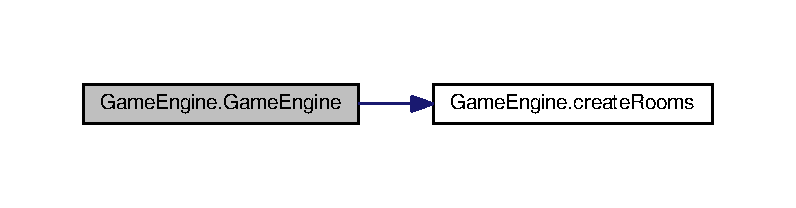
\includegraphics[width=350pt]{classGameEngine_a9e8a92f5021a34293060f9aaff4005de_cgraph}
\end{center}
\end{figure}




\subsection{Member Function Documentation}
\hypertarget{classGameEngine_a9410d92f7d0e6820059b1d07da364b09}{\index{Game\-Engine@{Game\-Engine}!create\-Rooms@{create\-Rooms}}
\index{create\-Rooms@{create\-Rooms}!GameEngine@{Game\-Engine}}
\subsubsection[{create\-Rooms}]{\setlength{\rightskip}{0pt plus 5cm}{\bf Room} Game\-Engine.\-create\-Rooms (
\begin{DoxyParamCaption}
{}
\end{DoxyParamCaption}
)\hspace{0.3cm}{\ttfamily [private]}}}\label{classGameEngine_a9410d92f7d0e6820059b1d07da364b09}


Create the rooms, link them and return the first \hyperlink{classRoom}{Room}. 

\begin{DoxyReturn}{Returns}
\hyperlink{classRoom}{Room} The first \hyperlink{classRoom}{Room} where the player should ba at start. 
\end{DoxyReturn}


Definition at line \hyperlink{GameEngine_8java_source_l00085}{85} of file \hyperlink{GameEngine_8java_source}{Game\-Engine.\-java}.



Referenced by \hyperlink{GameEngine_8java_source_l00047}{Game\-Engine()}.


\begin{DoxyCode}
00085                                \{
00086         \textcolor{comment}{// create the rooms}
00087         \hyperlink{classRoom}{Room} temperateBroadleaf = \textcolor{keyword}{new} \hyperlink{classRoom}{Room}(\textcolor{stringliteral}{"in temperate forest"}, \textcolor{stringliteral}{"temperatebroadleaf.jpg"});
00088         temperateBroadleaf.addItem(\textcolor{keyword}{new} \hyperlink{classItem}{Item}(\textcolor{stringliteral}{"wand"}, 3, \textcolor{stringliteral}{"just an ordinary wand"}));
00089 
00090         \hyperlink{classRoom}{Room} taiga = \textcolor{keyword}{new} \hyperlink{classRoom}{Room}(\textcolor{stringliteral}{"in a boreal forest"}, \textcolor{stringliteral}{"taiga.jpg"});
00091         taiga.addItem(\textcolor{keyword}{new} \hyperlink{classItem}{Item}(\textcolor{stringliteral}{"snowball"}, 1, \textcolor{stringliteral}{"some weirdly yellowy snowball"}));
00092         taiga.addItem(\textcolor{keyword}{new} \hyperlink{classItem}{Item}(\textcolor{stringliteral}{"bird"}, 6, \textcolor{stringliteral}{"a frozen inert black bird"}));
00093 
00094         \hyperlink{classRoom}{Room} alpineTundra = \textcolor{keyword}{new} \hyperlink{classRoom}{Room}(\textcolor{stringliteral}{"on an alpine mountain"}, \textcolor{stringliteral}{"alpinetundra.jpg"});
00095         alpineTundra.addItem(\textcolor{keyword}{new} \hyperlink{classItem}{Item}(\textcolor{stringliteral}{"rock"}, 15, \textcolor{stringliteral}{"a surprisingly solid magnificent rock"}));
00096         alpineTundra.addItem(\textcolor{keyword}{new} \hyperlink{classItem}{Item}(\textcolor{stringliteral}{"plank"}, 10, \textcolor{stringliteral}{"a plank of wood, maybe from a chalet"}));
00097         alpineTundra.addItem(\textcolor{keyword}{new} \hyperlink{classItem}{Item}(\textcolor{stringliteral}{"snowball"}, 1, \textcolor{stringliteral}{"a snowball. Yes, there is still snow in an alpine
       biome."}));
00098 
00099         \hyperlink{classRoom}{Room} steppe = \textcolor{keyword}{new} \hyperlink{classRoom}{Room}(\textcolor{stringliteral}{"on a vast grass plain"}, \textcolor{stringliteral}{"steppe.jpg"});
00100         steppe.addItem(\textcolor{keyword}{new} \hyperlink{classItem}{Item}(\textcolor{stringliteral}{"grass"}, 1, \textcolor{stringliteral}{"a tuft of yellowish grass. Looking at the grass made you
       look like stupid"}));
00101 
00102         \hyperlink{classRoom}{Room} cave = \textcolor{keyword}{new} \hyperlink{classRoom}{Room}(\textcolor{stringliteral}{"inside a dark cave"}, \textcolor{stringliteral}{"cave.jpg"});
00103         cave.addItem(\textcolor{keyword}{new} \hyperlink{classItem}{Item}(\textcolor{stringliteral}{"magiccookie"}, 3, \textcolor{stringliteral}{"a pretend magic cookie with mould on it, probably left
       there for many years. The use-by date has faded out. Why not eat it?"}));
00104 
00105         \hyperlink{classRoom}{Room} polarDesert = \textcolor{keyword}{new} \hyperlink{classRoom}{Room}(\textcolor{stringliteral}{"in a cold polar desert"}, \textcolor{stringliteral}{"polardesert.jpg"});
00106         polarDesert.addItem(\textcolor{keyword}{new} \hyperlink{classItem}{Item}(\textcolor{stringliteral}{"ice"}, 5, \textcolor{stringliteral}{"a little block of ice. But you don't have any drink"}));
00107 
00108         \hyperlink{classRoom}{Room} xericShrublands = \textcolor{keyword}{new} \hyperlink{classRoom}{Room}(\textcolor{stringliteral}{"in a sand desert"}, \textcolor{stringliteral}{"xericshrublands.jpg"});
00109         xericShrublands.addItem(\textcolor{keyword}{new} \hyperlink{classItem}{Item}(\textcolor{stringliteral}{"shrub"}, 10, \textcolor{stringliteral}{"a spicky shrub. Useful if you want to make a
       shruberry"}));
00110 
00111         \hyperlink{classRoom}{Room} savanna = \textcolor{keyword}{new} \hyperlink{classRoom}{Room}(\textcolor{stringliteral}{"in a savanna"}, \textcolor{stringliteral}{"savanna.jpg"});
00112         savanna.addItem(\textcolor{keyword}{new} \hyperlink{classItem}{Item}(\textcolor{stringliteral}{"elephant"}, 1000, \textcolor{stringliteral}{"a huge elephant looking at you, dazed. I bet he's
       smarter than you"}));
00113         savanna.addItem(\textcolor{keyword}{new} \hyperlink{classItem}{Item}(\textcolor{stringliteral}{"grass"}, 1, \textcolor{stringliteral}{"a tuft of yellowish grass. You may have other things to
       do instead of looking at that"}));
00114 
00115         \textcolor{comment}{// initialise room exits}
00116         temperateBroadleaf.setExit(\textcolor{stringliteral}{"east"}, taiga);
00117         temperateBroadleaf.setExit(\textcolor{stringliteral}{"south"}, steppe);
00118 
00119         taiga.setExit(\textcolor{stringliteral}{"west"}, temperateBroadleaf);
00120         taiga.setExit(\textcolor{stringliteral}{"east"}, alpineTundra);
00121         taiga.setExit(\textcolor{stringliteral}{"south"}, cave);
00122 
00123         alpineTundra.setExit(\textcolor{stringliteral}{"west"}, taiga);
00124         alpineTundra.setExit(\textcolor{stringliteral}{"south"}, polarDesert);
00125 
00126         steppe.setExit(\textcolor{stringliteral}{"north"}, temperateBroadleaf);
00127         steppe.setExit(\textcolor{stringliteral}{"east"}, cave);
00128         steppe.setExit(\textcolor{stringliteral}{"south"}, xericShrublands);
00129 
00130         cave.setExit(\textcolor{stringliteral}{"north"}, taiga);
00131         cave.setExit(\textcolor{stringliteral}{"south"}, savanna);
00132         cave.setExit(\textcolor{stringliteral}{"east"}, polarDesert);
00133         cave.setExit(\textcolor{stringliteral}{"west"}, steppe);
00134 
00135         \textcolor{comment}{// Trap Door}
00136         \textcolor{comment}{// polarDesert.setExit("north", alpineTundra);}
00137         polarDesert.setExit(\textcolor{stringliteral}{"west"}, cave);
00138 
00139         xericShrublands.setExit(\textcolor{stringliteral}{"north"}, steppe);
00140         xericShrublands.setExit(\textcolor{stringliteral}{"east"}, savanna);
00141 
00142         savanna.setExit(\textcolor{stringliteral}{"north"}, cave);
00143         savanna.setExit(\textcolor{stringliteral}{"west"}, xericShrublands);
00144 
00145         \hyperlink{classRoom}{Room} randomRoom = \textcolor{keyword}{new} \hyperlink{classRoom}{Room}(\textcolor{stringliteral}{""}, \textcolor{stringliteral}{""});
00146 
00147         polarDesert.setExit(\textcolor{stringliteral}{"south"}, randomRoom);
00148         savanna.setExit(\textcolor{stringliteral}{"east"}, randomRoom);
00149 
00150         gameRooms.add(randomRoom);
00151         gameRooms.add(temperateBroadleaf);
00152         gameRooms.add(taiga);
00153         gameRooms.add(alpineTundra);
00154         gameRooms.add(steppe);
00155         gameRooms.add(cave);
00156         gameRooms.add(polarDesert);
00157         gameRooms.add(xericShrublands);
00158         gameRooms.add(savanna);
00159 
00160         \textcolor{keywordflow}{return} temperateBroadleaf;
00161     \}
\end{DoxyCode}


Here is the caller graph for this function\-:
\nopagebreak
\begin{figure}[H]
\begin{center}
\leavevmode
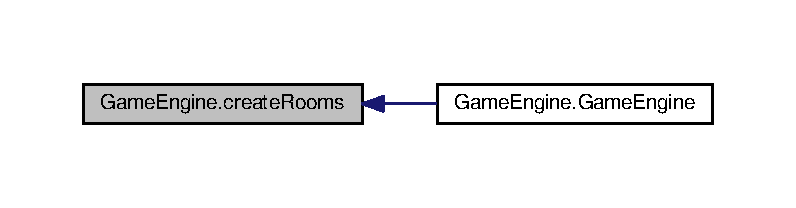
\includegraphics[width=350pt]{classGameEngine_a9410d92f7d0e6820059b1d07da364b09_icgraph}
\end{center}
\end{figure}


\hypertarget{classGameEngine_a1f5fa36c5dfc36c9a963fe439afc057b}{\index{Game\-Engine@{Game\-Engine}!end\-Game@{end\-Game}}
\index{end\-Game@{end\-Game}!GameEngine@{Game\-Engine}}
\subsubsection[{end\-Game}]{\setlength{\rightskip}{0pt plus 5cm}void Game\-Engine.\-end\-Game (
\begin{DoxyParamCaption}
\item[{boolean}]{winning}
\end{DoxyParamCaption}
)\hspace{0.3cm}{\ttfamily [private]}}}\label{classGameEngine_a1f5fa36c5dfc36c9a963fe439afc057b}


Print goodbye message and disable gui. 


\begin{DoxyParams}{Parameters}
{\em winning} & Equals to true if the player won \\
\hline
\end{DoxyParams}


Definition at line \hyperlink{GameEngine_8java_source_l00213}{213} of file \hyperlink{GameEngine_8java_source}{Game\-Engine.\-java}.



Referenced by \hyperlink{GameEngine_8java_source_l00167}{process\-Command()}.


\begin{DoxyCode}
00213                                           \{
00214         gui.println(\textcolor{stringliteral}{"Thank you for playing. Good bye. By the way, you "}
00215                 + ((winning)? \textcolor{stringliteral}{"won"} : \textcolor{stringliteral}{"lost"}) + \textcolor{stringliteral}{"."});
00216         gui.enable(\textcolor{keyword}{false});
00217     \}
\end{DoxyCode}


Here is the caller graph for this function\-:
\nopagebreak
\begin{figure}[H]
\begin{center}
\leavevmode
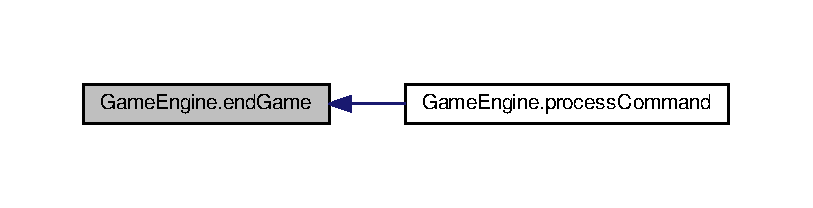
\includegraphics[width=350pt]{classGameEngine_a1f5fa36c5dfc36c9a963fe439afc057b_icgraph}
\end{center}
\end{figure}


\hypertarget{classGameEngine_a9a2f3cb921bb19399e357bf14d26425b}{\index{Game\-Engine@{Game\-Engine}!print\-Welcome@{print\-Welcome}}
\index{print\-Welcome@{print\-Welcome}!GameEngine@{Game\-Engine}}
\subsubsection[{print\-Welcome}]{\setlength{\rightskip}{0pt plus 5cm}void Game\-Engine.\-print\-Welcome (
\begin{DoxyParamCaption}
{}
\end{DoxyParamCaption}
)\hspace{0.3cm}{\ttfamily [private]}}}\label{classGameEngine_a9a2f3cb921bb19399e357bf14d26425b}


Welcome the user at the start of the game. 



Definition at line \hyperlink{GameEngine_8java_source_l00068}{68} of file \hyperlink{GameEngine_8java_source}{Game\-Engine.\-java}.



Referenced by \hyperlink{GameEngine_8java_source_l00059}{set\-G\-U\-I()}.


\begin{DoxyCode}
00068                                 \{
00069         gui.println(\textcolor{stringliteral}{"Greetings human."});
00070         gui.println(\textcolor{stringliteral}{"I see the assassins have failed. Too bad..."});
00071         gui.println(\textcolor{stringliteral}{"You know what they say: if you want something done, do it yourself."});
00072         gui.println(\textcolor{stringliteral}{"At least I can see that you don't remember anything. At last something that I can take
       advantage of."});
00073         gui.println(\textcolor{stringliteral}{"That was predictable, human minds are weak."});
00074         gui.println(\textcolor{stringliteral}{"\(\backslash\)nBecause you're stupid, I will describe you everything that will be around us."});
00075         gui.println(\textcolor{stringliteral}{"Who knows ? Maybe you can turn into something useful. One day. Maybe."});
00076         gui.println(\textcolor{stringliteral}{"\(\backslash\)nBeware: Death is coming!\(\backslash\)n"});
00077         gui.println(player.getCurrentRoom().getLongDescription());
00078         gui.showImage(player.getCurrentRoom().getImageName());
00079     \}
\end{DoxyCode}


Here is the caller graph for this function\-:
\nopagebreak
\begin{figure}[H]
\begin{center}
\leavevmode
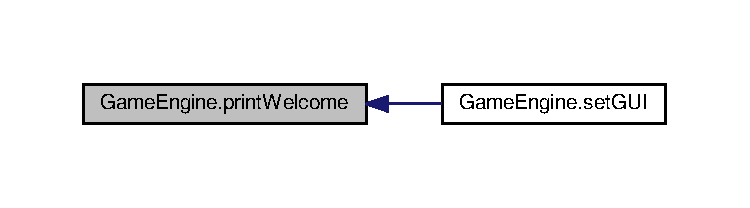
\includegraphics[width=350pt]{classGameEngine_a9a2f3cb921bb19399e357bf14d26425b_icgraph}
\end{center}
\end{figure}


\hypertarget{classGameEngine_ad7133885f313fa99bca3bb7cb8272f64}{\index{Game\-Engine@{Game\-Engine}!process\-Command@{process\-Command}}
\index{process\-Command@{process\-Command}!GameEngine@{Game\-Engine}}
\subsubsection[{process\-Command}]{\setlength{\rightskip}{0pt plus 5cm}void Game\-Engine.\-process\-Command (
\begin{DoxyParamCaption}
\item[{String}]{command\-Line}
\end{DoxyParamCaption}
)}}\label{classGameEngine_ad7133885f313fa99bca3bb7cb8272f64}


Process the command. 


\begin{DoxyParams}{Parameters}
{\em command\-Line} & The command to process. \\
\hline
\end{DoxyParams}


Definition at line \hyperlink{GameEngine_8java_source_l00167}{167} of file \hyperlink{GameEngine_8java_source}{Game\-Engine.\-java}.



References \hyperlink{GameEngine_8java_source_l00042}{command\-Count\-Down}, \hyperlink{GameEngine_8java_source_l00213}{end\-Game()}, \hyperlink{Player_8java_source_l00089}{Player.\-get\-Current\-Room()}, \hyperlink{GameEngine_8java_source_l00028}{gui}, \hyperlink{GameEngine_8java_source_l00018}{player}, and \hyperlink{UserInterface_8java_source_l00073}{User\-Interface.\-println()}.


\begin{DoxyCode}
00167                                                    \{
00168         gui.println(\textcolor{stringliteral}{"\(\backslash\)n"} + commandLine + \textcolor{stringliteral}{"\(\backslash\)n"});
00169         \hyperlink{classCommand}{Command} command = Parser.getCommand(commandLine);
00170 
00171         \textcolor{keywordflow}{if}(command == null) \{
00172             gui.println(\textcolor{stringliteral}{"I don't know what you mean..."});
00173             \textcolor{keywordflow}{return};
00174         \}
00175 
00176         gui.setCommandsLeft(--\hyperlink{classGameEngine_ad4ff8d760eced9c7b76cdeb0dc989975}{commandCountDown});
00177 
00178         \textcolor{keywordflow}{try} \{
00179             \textcolor{keywordtype}{boolean} quit = command.execute(\hyperlink{classGameEngine_a4666c6719428cc43014b30b305eeef5d}{player});
00180 
00181             \textcolor{keywordflow}{if}(command.hasMessage())
00182                 \hyperlink{classGameEngine_a2a7d0bb6183b3f3ef3ee2008926374a0}{gui}.\hyperlink{classUserInterface_a79f606b4b1f5d1523e50eea00039ed94}{println}(command.getMessage());
00183             \textcolor{comment}{// If we can cast the command into a GoCommand}
00184             \textcolor{comment}{// Or if it is the test command}
00185             \textcolor{keywordflow}{if}(\hyperlink{classGoCommand}{GoCommand}.class.isInstance(command) || command.getClass().equals(
      \hyperlink{classTestCommand}{TestCommand}.class)) \{
00186                 \textcolor{comment}{// The game image is reloaded}
00187                 \textcolor{keywordflow}{if}(\hyperlink{classGameEngine_a4666c6719428cc43014b30b305eeef5d}{player}.\hyperlink{classPlayer_a3a3107df50fc4e35e8c0f46c3f776ce6}{getCurrentRoom}().getImageName() != null) \{
00188                     gui.showImage(player.getCurrentRoom().getImageName());
00189                 \}
00190             \}
00191 
00192             \textcolor{keywordflow}{if}(quit) \{
00193                 \hyperlink{classGameEngine_a1f5fa36c5dfc36c9a963fe439afc057b}{endGame}(\textcolor{keyword}{false});
00194             \}
00195         \} \textcolor{keywordflow}{catch}(\hyperlink{classNoArgumentException}{NoArgumentException} e) \{
00196             gui.println(e.getMessage());
00197         \} \textcolor{keywordflow}{catch}(\hyperlink{classIllegalArgumentException}{IllegalArgumentException} e) \{
00198             gui.println(e.getMessage());
00199         \} \textcolor{keywordflow}{catch}(\hyperlink{classUnauthorizedException}{UnauthorizedException} e) \{
00200             gui.println(e.getMessage());
00201         \}
00202 
00203         \textcolor{keywordflow}{if}(\hyperlink{classGameEngine_ad4ff8d760eced9c7b76cdeb0dc989975}{commandCountDown} == 0) \{
00204             \hyperlink{classGameEngine_a1f5fa36c5dfc36c9a963fe439afc057b}{endGame}(\textcolor{keyword}{false});
00205         \}
00206 
00207     \}
\end{DoxyCode}


Here is the call graph for this function\-:
\nopagebreak
\begin{figure}[H]
\begin{center}
\leavevmode
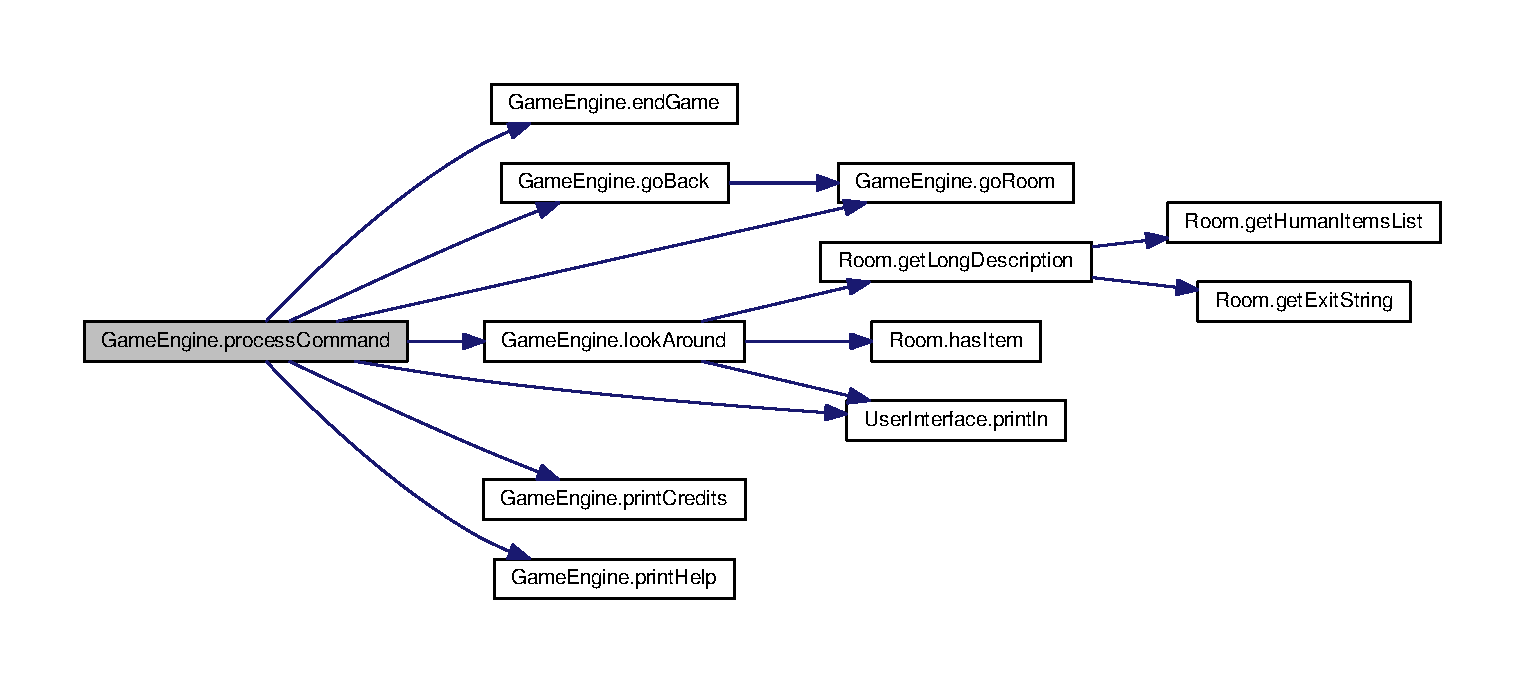
\includegraphics[width=350pt]{classGameEngine_ad7133885f313fa99bca3bb7cb8272f64_cgraph}
\end{center}
\end{figure}


\hypertarget{classGameEngine_aec901a5b590b3cd204f196165da5dfb6}{\index{Game\-Engine@{Game\-Engine}!set\-G\-U\-I@{set\-G\-U\-I}}
\index{set\-G\-U\-I@{set\-G\-U\-I}!GameEngine@{Game\-Engine}}
\subsubsection[{set\-G\-U\-I}]{\setlength{\rightskip}{0pt plus 5cm}void Game\-Engine.\-set\-G\-U\-I (
\begin{DoxyParamCaption}
\item[{{\bf User\-Interface}}]{user\-Interface}
\end{DoxyParamCaption}
)}}\label{classGameEngine_aec901a5b590b3cd204f196165da5dfb6}


Setter for the gui field. 


\begin{DoxyParams}{Parameters}
{\em user\-Interface} & The user interface to set \\
\hline
\end{DoxyParams}


Definition at line \hyperlink{GameEngine_8java_source_l00059}{59} of file \hyperlink{GameEngine_8java_source}{Game\-Engine.\-java}.



References \hyperlink{GameEngine_8java_source_l00042}{command\-Count\-Down}, \hyperlink{GameEngine_8java_source_l00028}{gui}, and \hyperlink{GameEngine_8java_source_l00068}{print\-Welcome()}.


\begin{DoxyCode}
00059                                                     \{
00060         \hyperlink{classGameEngine_a2a7d0bb6183b3f3ef3ee2008926374a0}{gui} = userInterface;
00061         gui.setCommandsLeft(\hyperlink{classGameEngine_ad4ff8d760eced9c7b76cdeb0dc989975}{commandCountDown});
00062         \hyperlink{classGameEngine_a9a2f3cb921bb19399e357bf14d26425b}{printWelcome}();
00063     \}
\end{DoxyCode}


Here is the call graph for this function\-:
\nopagebreak
\begin{figure}[H]
\begin{center}
\leavevmode
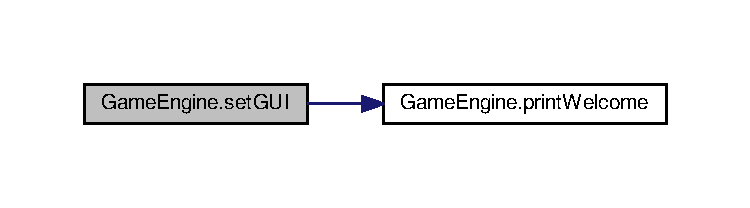
\includegraphics[width=350pt]{classGameEngine_aec901a5b590b3cd204f196165da5dfb6_cgraph}
\end{center}
\end{figure}




\subsection{Member Data Documentation}
\hypertarget{classGameEngine_ad4ff8d760eced9c7b76cdeb0dc989975}{\index{Game\-Engine@{Game\-Engine}!command\-Count\-Down@{command\-Count\-Down}}
\index{command\-Count\-Down@{command\-Count\-Down}!GameEngine@{Game\-Engine}}
\subsubsection[{command\-Count\-Down}]{\setlength{\rightskip}{0pt plus 5cm}int Game\-Engine.\-command\-Count\-Down\hspace{0.3cm}{\ttfamily [private]}}}\label{classGameEngine_ad4ff8d760eced9c7b76cdeb0dc989975}


The command number limit of the game. 

It is initially equals to 42 

Definition at line \hyperlink{GameEngine_8java_source_l00042}{42} of file \hyperlink{GameEngine_8java_source}{Game\-Engine.\-java}.



Referenced by \hyperlink{GameEngine_8java_source_l00047}{Game\-Engine()}, \hyperlink{GameEngine_8java_source_l00167}{process\-Command()}, and \hyperlink{GameEngine_8java_source_l00059}{set\-G\-U\-I()}.

\hypertarget{classGameEngine_ae5a2f252ec103e0630aebb8635341ea4}{\index{Game\-Engine@{Game\-Engine}!game\-Rooms@{game\-Rooms}}
\index{game\-Rooms@{game\-Rooms}!GameEngine@{Game\-Engine}}
\subsubsection[{game\-Rooms}]{\setlength{\rightskip}{0pt plus 5cm}Array\-List$<${\bf Room}$>$ Game\-Engine.\-game\-Rooms\hspace{0.3cm}{\ttfamily [package]}}}\label{classGameEngine_ae5a2f252ec103e0630aebb8635341ea4}


A list of all the rooms in the game. 



Definition at line \hyperlink{GameEngine_8java_source_l00023}{23} of file \hyperlink{GameEngine_8java_source}{Game\-Engine.\-java}.



Referenced by \hyperlink{GameEngine_8java_source_l00047}{Game\-Engine()}.

\hypertarget{classGameEngine_a2a7d0bb6183b3f3ef3ee2008926374a0}{\index{Game\-Engine@{Game\-Engine}!gui@{gui}}
\index{gui@{gui}!GameEngine@{Game\-Engine}}
\subsubsection[{gui}]{\setlength{\rightskip}{0pt plus 5cm}{\bf User\-Interface} Game\-Engine.\-gui\hspace{0.3cm}{\ttfamily [private]}}}\label{classGameEngine_a2a7d0bb6183b3f3ef3ee2008926374a0}


User interface for the game. 



Definition at line \hyperlink{GameEngine_8java_source_l00028}{28} of file \hyperlink{GameEngine_8java_source}{Game\-Engine.\-java}.



Referenced by \hyperlink{GameEngine_8java_source_l00167}{process\-Command()}, and \hyperlink{GameEngine_8java_source_l00059}{set\-G\-U\-I()}.

\hypertarget{classGameEngine_a308a9926d553d53cb4c56c28588f6c62}{\index{Game\-Engine@{Game\-Engine}!help\-Count@{help\-Count}}
\index{help\-Count@{help\-Count}!GameEngine@{Game\-Engine}}
\subsubsection[{help\-Count}]{\setlength{\rightskip}{0pt plus 5cm}int Game\-Engine.\-help\-Count\hspace{0.3cm}{\ttfamily [private]}}}\label{classGameEngine_a308a9926d553d53cb4c56c28588f6c62}


Help query counter. 

It is equal to 0 if the user did not asked for help, 1 if the user asked once the help and 2 if the user asked twice or more for the help 

Definition at line \hyperlink{GameEngine_8java_source_l00036}{36} of file \hyperlink{GameEngine_8java_source}{Game\-Engine.\-java}.



Referenced by \hyperlink{GameEngine_8java_source_l00047}{Game\-Engine()}.

\hypertarget{classGameEngine_a4666c6719428cc43014b30b305eeef5d}{\index{Game\-Engine@{Game\-Engine}!player@{player}}
\index{player@{player}!GameEngine@{Game\-Engine}}
\subsubsection[{player}]{\setlength{\rightskip}{0pt plus 5cm}{\bf Player} Game\-Engine.\-player\hspace{0.3cm}{\ttfamily [private]}}}\label{classGameEngine_a4666c6719428cc43014b30b305eeef5d}


\hyperlink{classPlayer}{Player} for the game. 



Definition at line \hyperlink{GameEngine_8java_source_l00018}{18} of file \hyperlink{GameEngine_8java_source}{Game\-Engine.\-java}.



Referenced by \hyperlink{GameEngine_8java_source_l00047}{Game\-Engine()}, and \hyperlink{GameEngine_8java_source_l00167}{process\-Command()}.



The documentation for this class was generated from the following file\-:\begin{DoxyCompactItemize}
\item 
\hyperlink{GameEngine_8java}{Game\-Engine.\-java}\end{DoxyCompactItemize}

\hypertarget{classItem}{\section{Item Class Reference}
\label{classItem}\index{Item@{Item}}
}


Collaboration diagram for Item\-:
\nopagebreak
\begin{figure}[H]
\begin{center}
\leavevmode
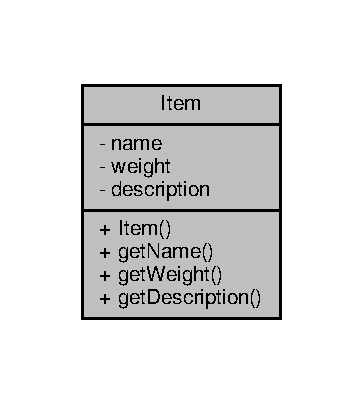
\includegraphics[width=174pt]{classItem__coll__graph}
\end{center}
\end{figure}
\subsection*{Public Member Functions}
\begin{DoxyCompactItemize}
\item 
\hyperlink{classItem_acf7048ce82d4f6f047d926b1f6260f7c}{Item} (String name, int weight, String description)
\item 
String \hyperlink{classItem_a78dd5a8370c5267c3f1f992167ab84ac}{get\-Name} ()
\item 
int \hyperlink{classItem_a2ff9daec3cf9585fb5741062447a779d}{get\-Weight} ()
\item 
String \hyperlink{classItem_abfe361bd046f5acdf4946bda076a8c8f}{get\-Description} ()
\end{DoxyCompactItemize}


\subsection{Detailed Description}
Class used to handle an item contained in a \hyperlink{classRoom}{Room}. \begin{DoxyAuthor}{Author}
Rémi Nicole 
\end{DoxyAuthor}


Definition at line \hyperlink{Item_8java_source_l00006}{6} of file \hyperlink{Item_8java_source}{Item.\-java}.



\subsection{Constructor \& Destructor Documentation}
\hypertarget{classItem_acf7048ce82d4f6f047d926b1f6260f7c}{\index{Item@{Item}!Item@{Item}}
\index{Item@{Item}!Item@{Item}}
\subsubsection[{Item}]{\setlength{\rightskip}{0pt plus 5cm}Item.\-Item (
\begin{DoxyParamCaption}
\item[{String}]{name, }
\item[{int}]{weight, }
\item[{String}]{description}
\end{DoxyParamCaption}
)}}\label{classItem_acf7048ce82d4f6f047d926b1f6260f7c}
\hyperlink{classItem}{Item} class constructor. 
\begin{DoxyParams}{Parameters}
{\em name} & Name of the item \\
\hline
{\em weight} & Weight of the item \\
\hline
{\em description} & Description of the item \\
\hline
\end{DoxyParams}


Definition at line \hyperlink{Item_8java_source_l00029}{29} of file \hyperlink{Item_8java_source}{Item.\-java}.


\begin{DoxyCode}
00029                                                              \{
00030         this.name = name;
00031         this.weight = weight;
00032         this.description = description;
00033     \}
\end{DoxyCode}


\subsection{Member Function Documentation}
\hypertarget{classItem_abfe361bd046f5acdf4946bda076a8c8f}{\index{Item@{Item}!get\-Description@{get\-Description}}
\index{get\-Description@{get\-Description}!Item@{Item}}
\subsubsection[{get\-Description}]{\setlength{\rightskip}{0pt plus 5cm}String Item.\-get\-Description (
\begin{DoxyParamCaption}
{}
\end{DoxyParamCaption}
)}}\label{classItem_abfe361bd046f5acdf4946bda076a8c8f}
description field getter. \begin{DoxyReturn}{Returns}
The description of the item 
\end{DoxyReturn}


Definition at line \hyperlink{Item_8java_source_l00055}{55} of file \hyperlink{Item_8java_source}{Item.\-java}.


\begin{DoxyCode}
00055                                    \{
00056         \textcolor{keywordflow}{return} description;
00057     \}
\end{DoxyCode}
\hypertarget{classItem_a78dd5a8370c5267c3f1f992167ab84ac}{\index{Item@{Item}!get\-Name@{get\-Name}}
\index{get\-Name@{get\-Name}!Item@{Item}}
\subsubsection[{get\-Name}]{\setlength{\rightskip}{0pt plus 5cm}String Item.\-get\-Name (
\begin{DoxyParamCaption}
{}
\end{DoxyParamCaption}
)}}\label{classItem_a78dd5a8370c5267c3f1f992167ab84ac}
name field getter. \begin{DoxyReturn}{Returns}
The name of the item 
\end{DoxyReturn}


Definition at line \hyperlink{Item_8java_source_l00039}{39} of file \hyperlink{Item_8java_source}{Item.\-java}.



Referenced by \hyperlink{Player_8java_source_l00186}{Player.\-take\-Object()}.


\begin{DoxyCode}
00039                             \{
00040         \textcolor{keywordflow}{return} name;
00041     \}
\end{DoxyCode}


Here is the caller graph for this function\-:
\nopagebreak
\begin{figure}[H]
\begin{center}
\leavevmode
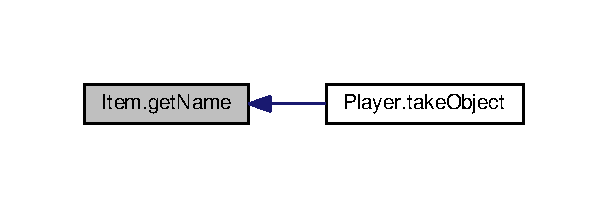
\includegraphics[width=292pt]{classItem_a78dd5a8370c5267c3f1f992167ab84ac_icgraph}
\end{center}
\end{figure}


\hypertarget{classItem_a2ff9daec3cf9585fb5741062447a779d}{\index{Item@{Item}!get\-Weight@{get\-Weight}}
\index{get\-Weight@{get\-Weight}!Item@{Item}}
\subsubsection[{get\-Weight}]{\setlength{\rightskip}{0pt plus 5cm}int Item.\-get\-Weight (
\begin{DoxyParamCaption}
{}
\end{DoxyParamCaption}
)}}\label{classItem_a2ff9daec3cf9585fb5741062447a779d}
weight field getter. \begin{DoxyReturn}{Returns}
The weight of the item 
\end{DoxyReturn}


Definition at line \hyperlink{Item_8java_source_l00047}{47} of file \hyperlink{Item_8java_source}{Item.\-java}.


\begin{DoxyCode}
00047                            \{
00048         \textcolor{keywordflow}{return} weight;
00049     \}
\end{DoxyCode}


The documentation for this class was generated from the following file\-:\begin{DoxyCompactItemize}
\item 
\hyperlink{Item_8java}{Item.\-java}\end{DoxyCompactItemize}

\hypertarget{classParser}{\section{Parser Class Reference}
\label{classParser}\index{Parser@{Parser}}
}


Collaboration diagram for Parser\-:
\nopagebreak
\begin{figure}[H]
\begin{center}
\leavevmode
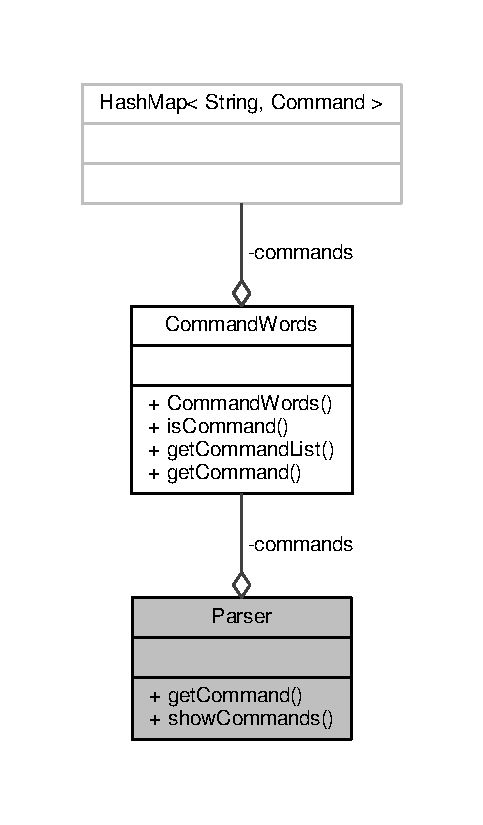
\includegraphics[width=187pt]{classParser__coll__graph}
\end{center}
\end{figure}
\subsection*{Public Member Functions}
\begin{DoxyCompactItemize}
\item 
\hyperlink{classParser_a5b20dc7a1c7a26ce3cec6cc070839bd4}{Parser} ()
\item 
Command \hyperlink{classParser_a5ee0a1ad3df67b8814d34c81e7276371}{get\-Command} (String input\-Line)
\item 
String \hyperlink{classParser_ae99d8549c08045804cc52576d7b4b453}{show\-Commands} ()
\end{DoxyCompactItemize}
\subsection*{Private Attributes}
\begin{DoxyCompactItemize}
\item 
\hyperlink{classCommandWords}{Command\-Words} \hyperlink{classParser_a6afb99e1595e6bc0705a09ee00dbddd6}{commands}
\end{DoxyCompactItemize}


\subsection{Detailed Description}
Class used to parse the commands with or without parameters given by the user.

\begin{DoxyAuthor}{Author}
Rémi N\-I\-C\-O\-L\-E 
\end{DoxyAuthor}


Definition at line \hyperlink{Parser_8java_source_l00009}{9} of file \hyperlink{Parser_8java_source}{Parser.\-java}.



\subsection{Constructor \& Destructor Documentation}
\hypertarget{classParser_a5b20dc7a1c7a26ce3cec6cc070839bd4}{\index{Parser@{Parser}!Parser@{Parser}}
\index{Parser@{Parser}!Parser@{Parser}}
\subsubsection[{Parser}]{\setlength{\rightskip}{0pt plus 5cm}Parser.\-Parser (
\begin{DoxyParamCaption}
{}
\end{DoxyParamCaption}
)}}\label{classParser_a5b20dc7a1c7a26ce3cec6cc070839bd4}
\hyperlink{classParser}{Parser} class constructor. 

Definition at line \hyperlink{Parser_8java_source_l00019}{19} of file \hyperlink{Parser_8java_source}{Parser.\-java}.



References \hyperlink{Parser_8java_source_l00014}{commands}.


\begin{DoxyCode}
00019                     \{
00020         \hyperlink{classParser_a6afb99e1595e6bc0705a09ee00dbddd6}{commands} = \textcolor{keyword}{new} \hyperlink{classCommandWords}{CommandWords}();
00021     \}
\end{DoxyCode}


\subsection{Member Function Documentation}
\hypertarget{classParser_a5ee0a1ad3df67b8814d34c81e7276371}{\index{Parser@{Parser}!get\-Command@{get\-Command}}
\index{get\-Command@{get\-Command}!Parser@{Parser}}
\subsubsection[{get\-Command}]{\setlength{\rightskip}{0pt plus 5cm}Command Parser.\-get\-Command (
\begin{DoxyParamCaption}
\item[{String}]{input\-Line}
\end{DoxyParamCaption}
)}}\label{classParser_a5ee0a1ad3df67b8814d34c81e7276371}
Get a new command from the user. 

Definition at line \hyperlink{Parser_8java_source_l00026}{26} of file \hyperlink{Parser_8java_source}{Parser.\-java}.



References \hyperlink{Parser_8java_source_l00014}{commands}, and \hyperlink{CommandWords_8java_source_l00028}{Command\-Words.\-is\-Command()}.


\begin{DoxyCode}
00026                                                 \{
00027 
00028         String word1;
00029         String word2;
00030 
00031         StringTokenizer tokenizer = \textcolor{keyword}{new} StringTokenizer(inputLine);
00032 
00033         \textcolor{keywordflow}{if}(tokenizer.hasMoreTokens())
00034             word1 = tokenizer.nextToken();  \textcolor{comment}{// First word}
00035         \textcolor{keywordflow}{else}
00036             word1 = null;
00037         \textcolor{keywordflow}{if}(tokenizer.hasMoreTokens())
00038             word2 = tokenizer.nextToken();  \textcolor{comment}{// Second word}
00039         \textcolor{keywordflow}{else}
00040             word2 = null;
00041 
00042         \textcolor{keywordflow}{if}(\hyperlink{classParser_a6afb99e1595e6bc0705a09ee00dbddd6}{commands}.\hyperlink{classCommandWords_a98619d278b3fa23fed18b5834f9d20a8}{isCommand}(word1))
00043             \textcolor{keywordflow}{return} \textcolor{keyword}{new} Command(word1, word2);
00044         \textcolor{keywordflow}{else}
00045             \textcolor{keywordflow}{return} \textcolor{keyword}{new} Command(null, word2);
00046     \}
\end{DoxyCode}


Here is the call graph for this function\-:\nopagebreak
\begin{figure}[H]
\begin{center}
\leavevmode
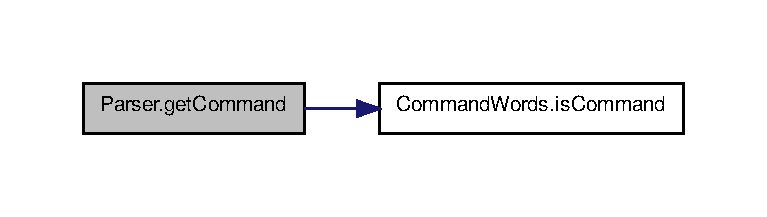
\includegraphics[width=350pt]{classParser_a5ee0a1ad3df67b8814d34c81e7276371_cgraph}
\end{center}
\end{figure}


\hypertarget{classParser_ae99d8549c08045804cc52576d7b4b453}{\index{Parser@{Parser}!show\-Commands@{show\-Commands}}
\index{show\-Commands@{show\-Commands}!Parser@{Parser}}
\subsubsection[{show\-Commands}]{\setlength{\rightskip}{0pt plus 5cm}String Parser.\-show\-Commands (
\begin{DoxyParamCaption}
{}
\end{DoxyParamCaption}
)}}\label{classParser_ae99d8549c08045804cc52576d7b4b453}
Getter for the known\-Commands field of the commands field. \begin{DoxySeeAlso}{See Also}
\hyperlink{classCommandWords_a328bb081d9a9e5cb1aa6362523b28783}{Command\-Words\-::known\-Commands} 
\end{DoxySeeAlso}


Definition at line \hyperlink{Parser_8java_source_l00052}{52} of file \hyperlink{Parser_8java_source}{Parser.\-java}.


\begin{DoxyCode}
00052                                  \{
00053         \textcolor{keywordflow}{return} commands.getCommandList();
00054     \}
\end{DoxyCode}


\subsection{Member Data Documentation}
\hypertarget{classParser_a6afb99e1595e6bc0705a09ee00dbddd6}{\index{Parser@{Parser}!commands@{commands}}
\index{commands@{commands}!Parser@{Parser}}
\subsubsection[{commands}]{\setlength{\rightskip}{0pt plus 5cm}{\bf Command\-Words} Parser.\-commands\hspace{0.3cm}{\ttfamily [private]}}}\label{classParser_a6afb99e1595e6bc0705a09ee00dbddd6}
Field used to get the list of known commands. 

Definition at line \hyperlink{Parser_8java_source_l00014}{14} of file \hyperlink{Parser_8java_source}{Parser.\-java}.



Referenced by \hyperlink{Parser_8java_source_l00026}{get\-Command()}, and \hyperlink{Parser_8java_source_l00019}{Parser()}.



The documentation for this class was generated from the following file\-:\begin{DoxyCompactItemize}
\item 
\hyperlink{Parser_8java}{Parser.\-java}\end{DoxyCompactItemize}

\hypertarget{classRoom}{\section{Room Class Reference}
\label{classRoom}\index{Room@{Room}}
}


Collaboration diagram for Room\-:
\nopagebreak
\begin{figure}[H]
\begin{center}
\leavevmode
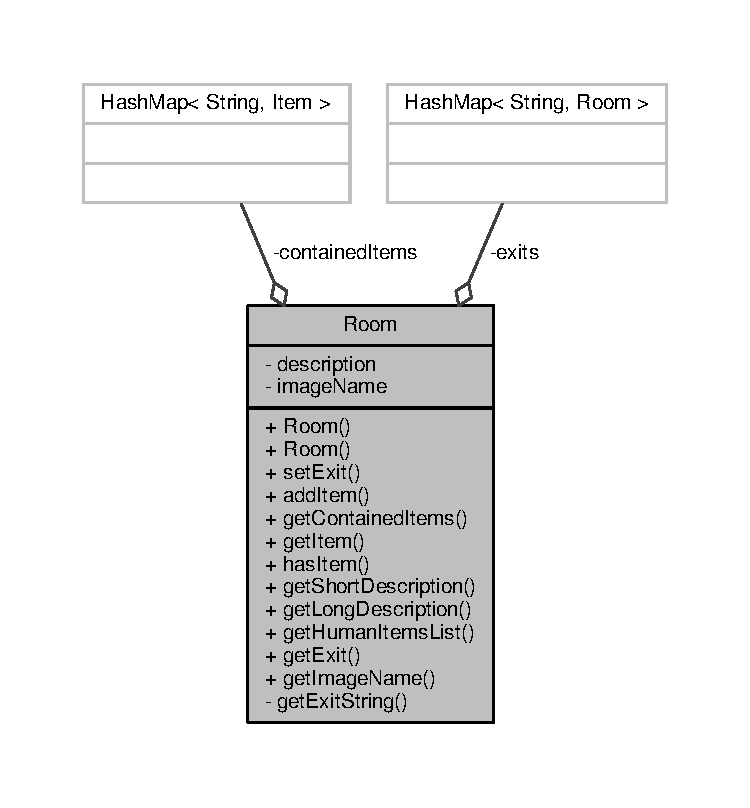
\includegraphics[width=198pt]{classRoom__coll__graph}
\end{center}
\end{figure}
\subsection*{Public Member Functions}
\begin{DoxyCompactItemize}
\item 
\hyperlink{classRoom_a2cdcbb3d86746330a5a01c7fae4de02c}{Room} (String description, String image)
\item 
\hyperlink{classRoom_a05e162f8831368304aa193ad5a05750c}{Room} (String description, String image, Hash\-Map$<$ String, \hyperlink{classItem}{Item} $>$ item\-List)
\item 
void \hyperlink{classRoom_ae4bc6837f331b5249beb0651fc277018}{set\-Exit} (String direction, \hyperlink{classRoom}{Room} neighbor)
\item 
void \hyperlink{classRoom_a0b4fcc1c1c04e60efa7ae5f82ea37157}{add\-Item} (\hyperlink{classItem}{Item} item)
\item 
Hash\-Map$<$ String, \hyperlink{classItem}{Item} $>$ \hyperlink{classRoom_a4d50f61fe592736e56e9e083b124ff83}{get\-Contained\-Items} ()
\item 
\hyperlink{classItem}{Item} \hyperlink{classRoom_a9b53c8d9f87f4a6d9cc954aeb744d1a2}{get\-Item} (String name)
\item 
boolean \hyperlink{classRoom_ad779b367b26018c9f343ca3044c4b54f}{has\-Item} (String name)
\item 
String \hyperlink{classRoom_a85e561bc5fa9d9c965300e9ad264b02a}{get\-Short\-Description} ()
\item 
String \hyperlink{classRoom_a23a25854d7544fb0b41190a4d6bd1322}{get\-Long\-Description} ()
\item 
String \hyperlink{classRoom_ab8a87ad306f77a936873094b479bcde8}{get\-Human\-Items\-List} ()
\item 
\hyperlink{classRoom}{Room} \hyperlink{classRoom_a384ab8c844e5775f87de24d6c470637e}{get\-Exit} (String direction)
\item 
String \hyperlink{classRoom_a8177668df4d8be718812934673c42649}{get\-Image\-Name} ()
\end{DoxyCompactItemize}


\subsection{Detailed Description}
Class used to handle a game's room. \begin{DoxyAuthor}{Author}
Rémi N\-I\-C\-O\-L\-E 
\end{DoxyAuthor}


Definition at line \hyperlink{Room_8java_source_l00011}{11} of file \hyperlink{Room_8java_source}{Room.\-java}.



\subsection{Constructor \& Destructor Documentation}
\hypertarget{classRoom_a2cdcbb3d86746330a5a01c7fae4de02c}{\index{Room@{Room}!Room@{Room}}
\index{Room@{Room}!Room@{Room}}
\subsubsection[{Room}]{\setlength{\rightskip}{0pt plus 5cm}Room.\-Room (
\begin{DoxyParamCaption}
\item[{String}]{description, }
\item[{String}]{image}
\end{DoxyParamCaption}
)}}\label{classRoom_a2cdcbb3d86746330a5a01c7fae4de02c}
\hyperlink{classRoom}{Room} class constructor. 
\begin{DoxyParams}{Parameters}
{\em description} & Description for the room \\
\hline
{\em image} & Image path to display \\
\hline
\end{DoxyParams}


Definition at line \hyperlink{Room_8java_source_l00039}{39} of file \hyperlink{Room_8java_source}{Room.\-java}.


\begin{DoxyCode}
00039                                                   \{
00040         \textcolor{keyword}{this}(description, image, \textcolor{keyword}{new} HashMap<String, Item>());
00041     \}
\end{DoxyCode}
\hypertarget{classRoom_a05e162f8831368304aa193ad5a05750c}{\index{Room@{Room}!Room@{Room}}
\index{Room@{Room}!Room@{Room}}
\subsubsection[{Room}]{\setlength{\rightskip}{0pt plus 5cm}Room.\-Room (
\begin{DoxyParamCaption}
\item[{String}]{description, }
\item[{String}]{image, }
\item[{Hash\-Map$<$ String, {\bf Item} $>$}]{item\-List}
\end{DoxyParamCaption}
)}}\label{classRoom_a05e162f8831368304aa193ad5a05750c}
\hyperlink{classRoom}{Room} class constructor with the items. 
\begin{DoxyParams}{Parameters}
{\em description} & Description for the room \\
\hline
{\em image} & Image path to display \\
\hline
{\em item\-List} & The items currently in the room \\
\hline
\end{DoxyParams}


Definition at line \hyperlink{Room_8java_source_l00049}{49} of file \hyperlink{Room_8java_source}{Room.\-java}.


\begin{DoxyCode}
00049                                                                                   \{
00050         this.description = description;
00051         exits = \textcolor{keyword}{new} HashMap < String, Room > ();
00052         imageName = image;
00053         containedItems = itemList;
00054     \}
\end{DoxyCode}


\subsection{Member Function Documentation}
\hypertarget{classRoom_a0b4fcc1c1c04e60efa7ae5f82ea37157}{\index{Room@{Room}!add\-Item@{add\-Item}}
\index{add\-Item@{add\-Item}!Room@{Room}}
\subsubsection[{add\-Item}]{\setlength{\rightskip}{0pt plus 5cm}void Room.\-add\-Item (
\begin{DoxyParamCaption}
\item[{{\bf Item}}]{item}
\end{DoxyParamCaption}
)}}\label{classRoom_a0b4fcc1c1c04e60efa7ae5f82ea37157}
Add an \hyperlink{classItem}{Item} in the \hyperlink{classRoom}{Room}. 

Definition at line \hyperlink{Room_8java_source_l00068}{68} of file \hyperlink{Room_8java_source}{Room.\-java}.


\begin{DoxyCode}
00068                                    \{
00069         containedItems.put(item.getName(), item);
00070     \}
\end{DoxyCode}
\hypertarget{classRoom_a4d50f61fe592736e56e9e083b124ff83}{\index{Room@{Room}!get\-Contained\-Items@{get\-Contained\-Items}}
\index{get\-Contained\-Items@{get\-Contained\-Items}!Room@{Room}}
\subsubsection[{get\-Contained\-Items}]{\setlength{\rightskip}{0pt plus 5cm}Hash\-Map$<$String, {\bf Item}$>$ Room.\-get\-Contained\-Items (
\begin{DoxyParamCaption}
{}
\end{DoxyParamCaption}
)}}\label{classRoom_a4d50f61fe592736e56e9e083b124ff83}
contained\-Item field getter. 

Definition at line \hyperlink{Room_8java_source_l00075}{75} of file \hyperlink{Room_8java_source}{Room.\-java}.


\begin{DoxyCode}
00075                                                      \{
00076         \textcolor{keywordflow}{return} containedItems;
00077     \}
\end{DoxyCode}
\hypertarget{classRoom_a384ab8c844e5775f87de24d6c470637e}{\index{Room@{Room}!get\-Exit@{get\-Exit}}
\index{get\-Exit@{get\-Exit}!Room@{Room}}
\subsubsection[{get\-Exit}]{\setlength{\rightskip}{0pt plus 5cm}{\bf Room} Room.\-get\-Exit (
\begin{DoxyParamCaption}
\item[{String}]{direction}
\end{DoxyParamCaption}
)}}\label{classRoom_a384ab8c844e5775f87de24d6c470637e}
Return the room in a specific direction. 
\begin{DoxyParams}{Parameters}
{\em direction} & The direction of the wanted room. \\
\hline
\end{DoxyParams}


Definition at line \hyperlink{Room_8java_source_l00148}{148} of file \hyperlink{Room_8java_source}{Room.\-java}.


\begin{DoxyCode}
00148                                           \{
00149         \textcolor{keywordflow}{return} exits.get(direction);
00150     \}
\end{DoxyCode}
\hypertarget{classRoom_ab8a87ad306f77a936873094b479bcde8}{\index{Room@{Room}!get\-Human\-Items\-List@{get\-Human\-Items\-List}}
\index{get\-Human\-Items\-List@{get\-Human\-Items\-List}!Room@{Room}}
\subsubsection[{get\-Human\-Items\-List}]{\setlength{\rightskip}{0pt plus 5cm}String Room.\-get\-Human\-Items\-List (
\begin{DoxyParamCaption}
{}
\end{DoxyParamCaption}
)}}\label{classRoom_ab8a87ad306f77a936873094b479bcde8}
Return a human readable list of the items in the room. \begin{DoxyReturn}{Returns}
String The list of the items 
\end{DoxyReturn}


Definition at line \hyperlink{Room_8java_source_l00110}{110} of file \hyperlink{Room_8java_source}{Room.\-java}.



Referenced by \hyperlink{Room_8java_source_l00100}{get\-Long\-Description()}.


\begin{DoxyCode}
00110                                       \{
00111         String itemsList = \textcolor{stringliteral}{""};
00112         Set<String> names = containedItems.keySet();
00113         Iterator<String> it = names.iterator();
00114         \textcolor{keywordflow}{while}(it.hasNext()) \{
00115 
00116             String itemName = it.next();
00117             \textcolor{comment}{// If the item's name begins with a vowel, the prefix is ' an '}
00118             \textcolor{comment}{// if not, the prefix is ' a '}
00119             String prefix = \textcolor{stringliteral}{" a"} + (((\textcolor{keyword}{new} String(\textcolor{stringliteral}{"aeiouy"})).contains(itemName.substring(0,1)))? \textcolor{stringliteral}{"n"} : \textcolor{stringliteral}{""}) +
       \textcolor{stringliteral}{" "};
00120 
00121             \textcolor{keywordflow}{if}(itemsList.equals(\textcolor{stringliteral}{""}))
00122                 itemsList += prefix + itemName;
00123             \textcolor{keywordflow}{else} \{
00124                 \textcolor{comment}{// Check if it is the last item}
00125                 \textcolor{keywordflow}{if}(it.hasNext())
00126                     itemsList += \textcolor{stringliteral}{","} + prefix + itemName;
00127                 \textcolor{keywordflow}{else}
00128                     itemsList += \textcolor{stringliteral}{" and"} + prefix + itemName;
00129             \}
00130         \}
00131         \textcolor{keywordflow}{return} itemsList;
00132     \}
\end{DoxyCode}


Here is the caller graph for this function\-:
\nopagebreak
\begin{figure}[H]
\begin{center}
\leavevmode
\includegraphics[width=350pt]{classRoom_ab8a87ad306f77a936873094b479bcde8_icgraph}
\end{center}
\end{figure}


\hypertarget{classRoom_a8177668df4d8be718812934673c42649}{\index{Room@{Room}!get\-Image\-Name@{get\-Image\-Name}}
\index{get\-Image\-Name@{get\-Image\-Name}!Room@{Room}}
\subsubsection[{get\-Image\-Name}]{\setlength{\rightskip}{0pt plus 5cm}String Room.\-get\-Image\-Name (
\begin{DoxyParamCaption}
{}
\end{DoxyParamCaption}
)}}\label{classRoom_a8177668df4d8be718812934673c42649}
Getter for the image\-Name field. 

Definition at line \hyperlink{Room_8java_source_l00155}{155} of file \hyperlink{Room_8java_source}{Room.\-java}.


\begin{DoxyCode}
00155                                  \{
00156         \textcolor{keywordflow}{return} \textcolor{stringliteral}{"Images/"}  + imageName;
00157     \}
\end{DoxyCode}
\hypertarget{classRoom_a9b53c8d9f87f4a6d9cc954aeb744d1a2}{\index{Room@{Room}!get\-Item@{get\-Item}}
\index{get\-Item@{get\-Item}!Room@{Room}}
\subsubsection[{get\-Item}]{\setlength{\rightskip}{0pt plus 5cm}{\bf Item} Room.\-get\-Item (
\begin{DoxyParamCaption}
\item[{String}]{name}
\end{DoxyParamCaption}
)}}\label{classRoom_a9b53c8d9f87f4a6d9cc954aeb744d1a2}


Definition at line \hyperlink{Room_8java_source_l00079}{79} of file \hyperlink{Room_8java_source}{Room.\-java}.


\begin{DoxyCode}
00079                                      \{
00080         \textcolor{keywordflow}{return} containedItems.get(name);
00081     \}
\end{DoxyCode}
\hypertarget{classRoom_a23a25854d7544fb0b41190a4d6bd1322}{\index{Room@{Room}!get\-Long\-Description@{get\-Long\-Description}}
\index{get\-Long\-Description@{get\-Long\-Description}!Room@{Room}}
\subsubsection[{get\-Long\-Description}]{\setlength{\rightskip}{0pt plus 5cm}String Room.\-get\-Long\-Description (
\begin{DoxyParamCaption}
{}
\end{DoxyParamCaption}
)}}\label{classRoom_a23a25854d7544fb0b41190a4d6bd1322}
Return the description of the room, the available exits plus the items in the room if any. \begin{DoxyReturn}{Returns}
String The description. 
\end{DoxyReturn}


Definition at line \hyperlink{Room_8java_source_l00100}{100} of file \hyperlink{Room_8java_source}{Room.\-java}.



References \hyperlink{Room_8java_source_l00110}{get\-Human\-Items\-List()}.


\begin{DoxyCode}
00100                                        \{
00101         \textcolor{keywordflow}{return} \textcolor{stringliteral}{"You are "} + description + \textcolor{stringliteral}{".\(\backslash\)n"}
00102                 + ((!containedItems.isEmpty())? \textcolor{stringliteral}{"You can see"} + 
      \hyperlink{classRoom_ab8a87ad306f77a936873094b479bcde8}{getHumanItemsList}() + \textcolor{stringliteral}{" near you.\(\backslash\)n"} : \textcolor{stringliteral}{""})
00103                 + getExitString();
00104     \}
\end{DoxyCode}


Here is the call graph for this function\-:
\nopagebreak
\begin{figure}[H]
\begin{center}
\leavevmode
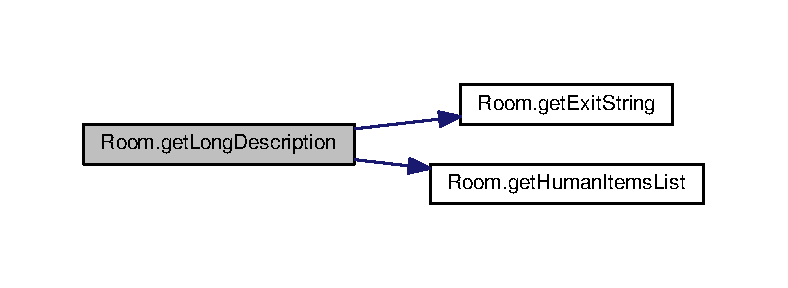
\includegraphics[width=350pt]{classRoom_a23a25854d7544fb0b41190a4d6bd1322_cgraph}
\end{center}
\end{figure}


\hypertarget{classRoom_a85e561bc5fa9d9c965300e9ad264b02a}{\index{Room@{Room}!get\-Short\-Description@{get\-Short\-Description}}
\index{get\-Short\-Description@{get\-Short\-Description}!Room@{Room}}
\subsubsection[{get\-Short\-Description}]{\setlength{\rightskip}{0pt plus 5cm}String Room.\-get\-Short\-Description (
\begin{DoxyParamCaption}
{}
\end{DoxyParamCaption}
)}}\label{classRoom_a85e561bc5fa9d9c965300e9ad264b02a}
Getter for the description field. \begin{DoxyReturn}{Returns}
String The description field 
\end{DoxyReturn}


Definition at line \hyperlink{Room_8java_source_l00091}{91} of file \hyperlink{Room_8java_source}{Room.\-java}.


\begin{DoxyCode}
00091                                         \{
00092         \textcolor{keywordflow}{return} description;
00093     \}
\end{DoxyCode}
\hypertarget{classRoom_ad779b367b26018c9f343ca3044c4b54f}{\index{Room@{Room}!has\-Item@{has\-Item}}
\index{has\-Item@{has\-Item}!Room@{Room}}
\subsubsection[{has\-Item}]{\setlength{\rightskip}{0pt plus 5cm}boolean Room.\-has\-Item (
\begin{DoxyParamCaption}
\item[{String}]{name}
\end{DoxyParamCaption}
)}}\label{classRoom_ad779b367b26018c9f343ca3044c4b54f}


Definition at line \hyperlink{Room_8java_source_l00083}{83} of file \hyperlink{Room_8java_source}{Room.\-java}.


\begin{DoxyCode}
00083                                         \{
00084         \textcolor{keywordflow}{return} containedItems.get(name) != null;
00085     \}
\end{DoxyCode}
\hypertarget{classRoom_ae4bc6837f331b5249beb0651fc277018}{\index{Room@{Room}!set\-Exit@{set\-Exit}}
\index{set\-Exit@{set\-Exit}!Room@{Room}}
\subsubsection[{set\-Exit}]{\setlength{\rightskip}{0pt plus 5cm}void Room.\-set\-Exit (
\begin{DoxyParamCaption}
\item[{String}]{direction, }
\item[{{\bf Room}}]{neighbor}
\end{DoxyParamCaption}
)}}\label{classRoom_ae4bc6837f331b5249beb0651fc277018}
Define a room in a relative direction to the current room. 
\begin{DoxyParams}{Parameters}
{\em direction} & Direction in which the room is. \\
\hline
{\em neighbor} & The room in that direction. \\
\hline
\end{DoxyParams}


Definition at line \hyperlink{Room_8java_source_l00061}{61} of file \hyperlink{Room_8java_source}{Room.\-java}.


\begin{DoxyCode}
00061                                                          \{
00062         exits.put(direction, neighbor);
00063     \}
\end{DoxyCode}


The documentation for this class was generated from the following file\-:\begin{DoxyCompactItemize}
\item 
\hyperlink{Room_8java}{Room.\-java}\end{DoxyCompactItemize}

\hypertarget{classUserInterface}{\section{User\-Interface Class Reference}
\label{classUserInterface}\index{User\-Interface@{User\-Interface}}
}


Inheritance diagram for User\-Interface\-:
\nopagebreak
\begin{figure}[H]
\begin{center}
\leavevmode
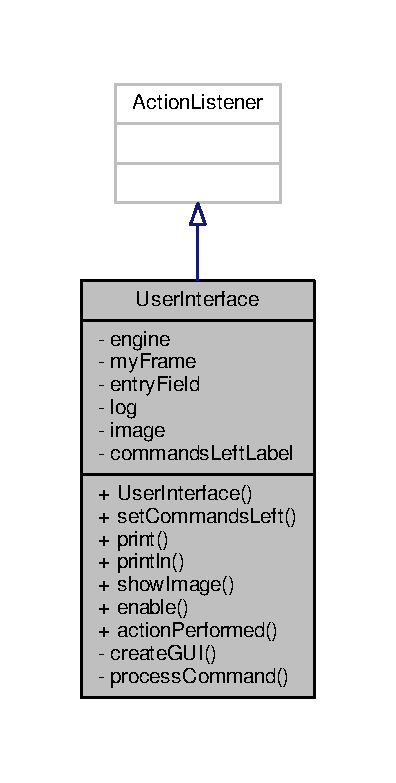
\includegraphics[width=190pt]{classUserInterface__inherit__graph}
\end{center}
\end{figure}


Collaboration diagram for User\-Interface\-:
\nopagebreak
\begin{figure}[H]
\begin{center}
\leavevmode
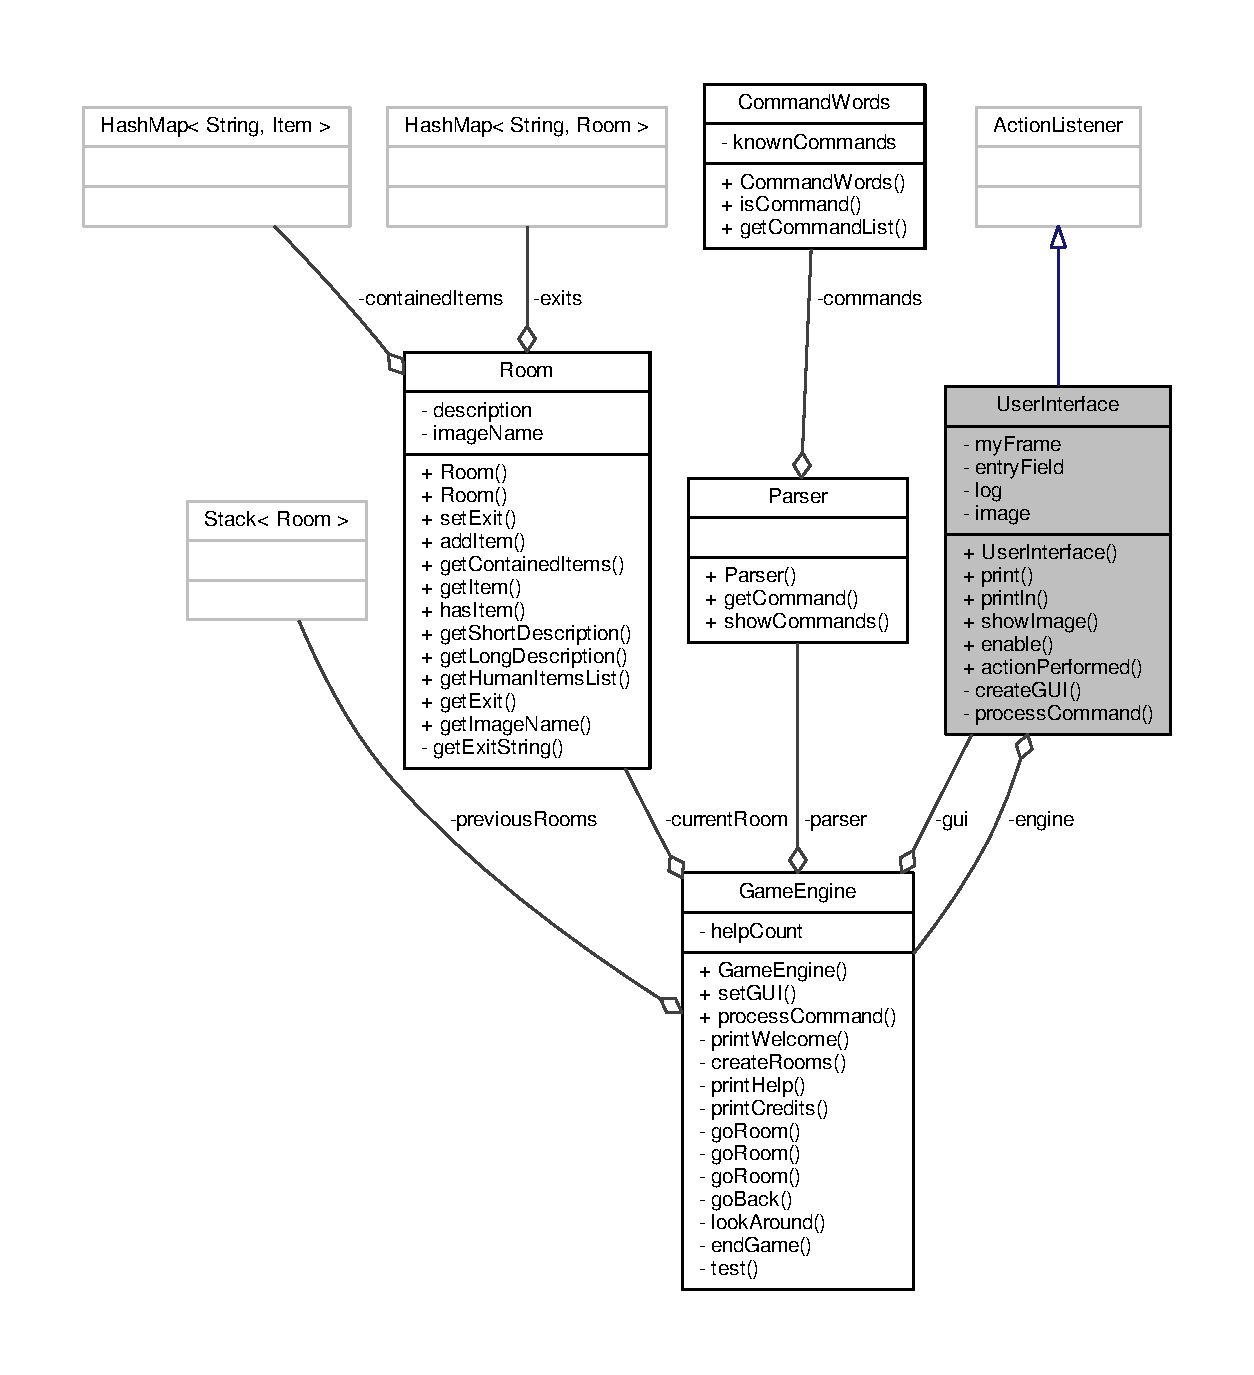
\includegraphics[width=190pt]{classUserInterface__coll__graph}
\end{center}
\end{figure}
\subsection*{Public Member Functions}
\begin{DoxyCompactItemize}
\item 
\hyperlink{classUserInterface_a3afe416f3ee335fec8bc815d382c3874}{User\-Interface} (\hyperlink{classGameEngine}{Game\-Engine} game\-Engine)
\item 
void \hyperlink{classUserInterface_ad12f31e49e7ed0904bc51ad330e55147}{set\-Commands\-Left} (int commands\-Left)
\item 
void \hyperlink{classUserInterface_a7a0de5ce2b0e0d25ba6573e87c63c1de}{print} (String text)
\item 
void \hyperlink{classUserInterface_a79f606b4b1f5d1523e50eea00039ed94}{println} (String text)
\item 
void \hyperlink{classUserInterface_ab793a0f12878c698ba3e1720a9f86f3b}{show\-Image} (String image\-Name)
\item 
void \hyperlink{classUserInterface_ab9e499c6c847d52c8753f08d62f1adfc}{enable} (boolean on)
\item 
void \hyperlink{classUserInterface_a0a1ee40a4dbca4aeee002c3d0537c7d5}{action\-Performed} (Action\-Event e)
\end{DoxyCompactItemize}


\subsection{Detailed Description}
Class handling the game's user interface. \begin{DoxyAuthor}{Author}
Rémi N\-I\-C\-O\-L\-E 
\end{DoxyAuthor}


Definition at line \hyperlink{UserInterface_8java_source_l00011}{11} of file \hyperlink{UserInterface_8java_source}{User\-Interface.\-java}.



\subsection{Constructor \& Destructor Documentation}
\hypertarget{classUserInterface_a3afe416f3ee335fec8bc815d382c3874}{\index{User\-Interface@{User\-Interface}!User\-Interface@{User\-Interface}}
\index{User\-Interface@{User\-Interface}!UserInterface@{User\-Interface}}
\subsubsection[{User\-Interface}]{\setlength{\rightskip}{0pt plus 5cm}User\-Interface.\-User\-Interface (
\begin{DoxyParamCaption}
\item[{{\bf Game\-Engine}}]{game\-Engine}
\end{DoxyParamCaption}
)}}\label{classUserInterface_a3afe416f3ee335fec8bc815d382c3874}
\hyperlink{classUserInterface}{User\-Interface} class constructor. 
\begin{DoxyParams}{Parameters}
{\em game\-Engine} & The gameplay \hyperlink{classGameEngine}{Game\-Engine} object. \\
\hline
\end{DoxyParams}


Definition at line \hyperlink{UserInterface_8java_source_l00047}{47} of file \hyperlink{UserInterface_8java_source}{User\-Interface.\-java}.


\begin{DoxyCode}
00047                                                 \{
00048         engine = gameEngine;
00049         createGUI();
00050     \}
\end{DoxyCode}


\subsection{Member Function Documentation}
\hypertarget{classUserInterface_a0a1ee40a4dbca4aeee002c3d0537c7d5}{\index{User\-Interface@{User\-Interface}!action\-Performed@{action\-Performed}}
\index{action\-Performed@{action\-Performed}!UserInterface@{User\-Interface}}
\subsubsection[{action\-Performed}]{\setlength{\rightskip}{0pt plus 5cm}void User\-Interface.\-action\-Performed (
\begin{DoxyParamCaption}
\item[{Action\-Event}]{e}
\end{DoxyParamCaption}
)}}\label{classUserInterface_a0a1ee40a4dbca4aeee002c3d0537c7d5}
Actionlistener for the textfield. 
\begin{DoxyParams}{Parameters}
{\em e} & Event \\
\hline
\end{DoxyParams}


Definition at line \hyperlink{UserInterface_8java_source_l00182}{182} of file \hyperlink{UserInterface_8java_source}{User\-Interface.\-java}.


\begin{DoxyCode}
00182                                                \{
00183         \textcolor{keywordflow}{if}(e.getActionCommand().equals(\textcolor{stringliteral}{"↑"})) \{
00184             engine.processCommand(\textcolor{stringliteral}{"go north"});
00185         \} \textcolor{keywordflow}{else} \textcolor{keywordflow}{if}(e.getActionCommand().equals(\textcolor{stringliteral}{"↓"})) \{
00186             engine.processCommand(\textcolor{stringliteral}{"go south"});
00187         \} \textcolor{keywordflow}{else} \textcolor{keywordflow}{if}(e.getActionCommand().equals(\textcolor{stringliteral}{"←"})) \{
00188             engine.processCommand(\textcolor{stringliteral}{"go west"});
00189         \} \textcolor{keywordflow}{else} \textcolor{keywordflow}{if}(e.getActionCommand().equals(\textcolor{stringliteral}{"→"})) \{
00190             engine.processCommand(\textcolor{stringliteral}{"go east"});
00191         \} \textcolor{keywordflow}{else} \textcolor{keywordflow}{if}(e.getActionCommand().equals(\textcolor{stringliteral}{"?"})) \{
00192             engine.processCommand(\textcolor{stringliteral}{"help"});
00193         \} \textcolor{keywordflow}{else} \{
00194             processCommand();
00195         \}
00196     \}
\end{DoxyCode}
\hypertarget{classUserInterface_ab9e499c6c847d52c8753f08d62f1adfc}{\index{User\-Interface@{User\-Interface}!enable@{enable}}
\index{enable@{enable}!UserInterface@{User\-Interface}}
\subsubsection[{enable}]{\setlength{\rightskip}{0pt plus 5cm}void User\-Interface.\-enable (
\begin{DoxyParamCaption}
\item[{boolean}]{on}
\end{DoxyParamCaption}
)}}\label{classUserInterface_ab9e499c6c847d52c8753f08d62f1adfc}
Enable or disable the input field. 
\begin{DoxyParams}{Parameters}
{\em on} & True to activate, False to deactivate \\
\hline
\end{DoxyParams}


Definition at line \hyperlink{UserInterface_8java_source_l00097}{97} of file \hyperlink{UserInterface_8java_source}{User\-Interface.\-java}.


\begin{DoxyCode}
00097                                    \{
00098         entryField.setEditable(on);
00099         \textcolor{keywordflow}{if}(!on)
00100             entryField.getCaret().setBlinkRate(0);
00101     \}
\end{DoxyCode}
\hypertarget{classUserInterface_a7a0de5ce2b0e0d25ba6573e87c63c1de}{\index{User\-Interface@{User\-Interface}!print@{print}}
\index{print@{print}!UserInterface@{User\-Interface}}
\subsubsection[{print}]{\setlength{\rightskip}{0pt plus 5cm}void User\-Interface.\-print (
\begin{DoxyParamCaption}
\item[{String}]{text}
\end{DoxyParamCaption}
)}}\label{classUserInterface_a7a0de5ce2b0e0d25ba6573e87c63c1de}
Print the given text in the text area. 
\begin{DoxyParams}{Parameters}
{\em text} & Text to display \\
\hline
\end{DoxyParams}


Definition at line \hyperlink{UserInterface_8java_source_l00064}{64} of file \hyperlink{UserInterface_8java_source}{User\-Interface.\-java}.


\begin{DoxyCode}
00064                                    \{
00065         log.append(text);
00066         log.setCaretPosition(log.getDocument().getLength());
00067     \}
\end{DoxyCode}
\hypertarget{classUserInterface_a79f606b4b1f5d1523e50eea00039ed94}{\index{User\-Interface@{User\-Interface}!println@{println}}
\index{println@{println}!UserInterface@{User\-Interface}}
\subsubsection[{println}]{\setlength{\rightskip}{0pt plus 5cm}void User\-Interface.\-println (
\begin{DoxyParamCaption}
\item[{String}]{text}
\end{DoxyParamCaption}
)}}\label{classUserInterface_a79f606b4b1f5d1523e50eea00039ed94}
Print the given text plus a newline in the text area. 
\begin{DoxyParams}{Parameters}
{\em text} & Text to display \\
\hline
\end{DoxyParams}


Definition at line \hyperlink{UserInterface_8java_source_l00073}{73} of file \hyperlink{UserInterface_8java_source}{User\-Interface.\-java}.



Referenced by \hyperlink{GameEngine_8java_source_l00167}{Game\-Engine.\-process\-Command()}.


\begin{DoxyCode}
00073                                      \{
00074         log.append(text + \textcolor{stringliteral}{"\(\backslash\)n"});
00075         log.setCaretPosition(log.getDocument().getLength());
00076     \}
\end{DoxyCode}


Here is the caller graph for this function\-:
\nopagebreak
\begin{figure}[H]
\begin{center}
\leavevmode
\includegraphics[width=350pt]{classUserInterface_a79f606b4b1f5d1523e50eea00039ed94_icgraph}
\end{center}
\end{figure}


\hypertarget{classUserInterface_ad12f31e49e7ed0904bc51ad330e55147}{\index{User\-Interface@{User\-Interface}!set\-Commands\-Left@{set\-Commands\-Left}}
\index{set\-Commands\-Left@{set\-Commands\-Left}!UserInterface@{User\-Interface}}
\subsubsection[{set\-Commands\-Left}]{\setlength{\rightskip}{0pt plus 5cm}void User\-Interface.\-set\-Commands\-Left (
\begin{DoxyParamCaption}
\item[{int}]{commands\-Left}
\end{DoxyParamCaption}
)}}\label{classUserInterface_ad12f31e49e7ed0904bc51ad330e55147}
Change the text for the commands left J\-Label 
\begin{DoxyParams}{Parameters}
{\em commands\-Left} & The number of commands left \\
\hline
\end{DoxyParams}


Definition at line \hyperlink{UserInterface_8java_source_l00056}{56} of file \hyperlink{UserInterface_8java_source}{User\-Interface.\-java}.


\begin{DoxyCode}
00056                                                   \{
00057         commandsLeftLabel.setText(\textcolor{stringliteral}{" Commands left: "} + commandsLeft + \textcolor{stringliteral}{"  "});
00058     \}
\end{DoxyCode}
\hypertarget{classUserInterface_ab793a0f12878c698ba3e1720a9f86f3b}{\index{User\-Interface@{User\-Interface}!show\-Image@{show\-Image}}
\index{show\-Image@{show\-Image}!UserInterface@{User\-Interface}}
\subsubsection[{show\-Image}]{\setlength{\rightskip}{0pt plus 5cm}void User\-Interface.\-show\-Image (
\begin{DoxyParamCaption}
\item[{String}]{image\-Name}
\end{DoxyParamCaption}
)}}\label{classUserInterface_ab793a0f12878c698ba3e1720a9f86f3b}
Show the image corresponding to the path of the image. 
\begin{DoxyParams}{Parameters}
{\em image\-Name} & The path of the image \\
\hline
\end{DoxyParams}


Definition at line \hyperlink{UserInterface_8java_source_l00082}{82} of file \hyperlink{UserInterface_8java_source}{User\-Interface.\-java}.


\begin{DoxyCode}
00082                                             \{
00083         URL imageURL = this.getClass().getClassLoader().getResource(imageName);
00084         \textcolor{keywordflow}{if}(imageURL == null)
00085             System.out.println(\textcolor{stringliteral}{"image not found"});
00086         \textcolor{keywordflow}{else} \{
00087             ImageIcon icon = \textcolor{keyword}{new} ImageIcon(imageURL);
00088             image.setIcon(icon);
00089             myFrame.pack();
00090         \}
00091     \}
\end{DoxyCode}


The documentation for this class was generated from the following file\-:\begin{DoxyCompactItemize}
\item 
\hyperlink{UserInterface_8java}{User\-Interface.\-java}\end{DoxyCompactItemize}

\chapter{File Documentation}
\hypertarget{Command_8java}{\section{Command.\-java File Reference}
\label{Command_8java}\index{Command.\-java@{Command.\-java}}
}
\subsection*{Classes}
\begin{DoxyCompactItemize}
\item 
class {\bfseries Command}
\end{DoxyCompactItemize}

\hypertarget{Command_8java}{\section{Command.\-java}
\label{Command_8java}\index{pkg\-\_\-commands/\-Command.\-java@{pkg\-\_\-commands/\-Command.\-java}}
}

\begin{DoxyCode}
00001 
00005 \textcolor{keyword}{package }pkg\_commands;
00006 
00007 \textcolor{keyword}{import} \hyperlink{classpkg__world_1_1Player}{pkg\_world.Player};
00008 \textcolor{keyword}{import} pkg\_exceptions.*;
00009 
\hypertarget{Command_8java_source_l00014}{}\hyperlink{classpkg__commands_1_1Command}{00014} \textcolor{keyword}{public} \textcolor{keyword}{abstract} \textcolor{keyword}{class }\hyperlink{classpkg__commands_1_1Command}{Command} \{
00015 
00021     \textcolor{keyword}{private} String parameter;
00022 
00028     \textcolor{keyword}{private} String secondParameter;
00029 
00035     \textcolor{keyword}{private} String message;
00036 
\hypertarget{Command_8java_source_l00041}{}\hyperlink{classpkg__commands_1_1Command_a41c92d445be73ea9d62320c65efb8434}{00041}     \textcolor{keyword}{public} String \hyperlink{classpkg__commands_1_1Command_a41c92d445be73ea9d62320c65efb8434}{getParameter}() \{
00042         \textcolor{keywordflow}{return} parameter;
00043     \}
00044 
\hypertarget{Command_8java_source_l00049}{}\hyperlink{classpkg__commands_1_1Command_a20d3ebdc0683a87b43be2a92a1cad111}{00049}     \textcolor{keyword}{public} String \hyperlink{classpkg__commands_1_1Command_a20d3ebdc0683a87b43be2a92a1cad111}{getSecondParameter}() \{
00050         \textcolor{keywordflow}{return} secondParameter;
00051     \}
00052 
\hypertarget{Command_8java_source_l00057}{}\hyperlink{classpkg__commands_1_1Command_a18446243a5fd360e9341b4b141c0cccc}{00057}     \textcolor{keyword}{public} \textcolor{keywordtype}{void} \hyperlink{classpkg__commands_1_1Command_a18446243a5fd360e9341b4b141c0cccc}{setParameter}(String parameter) \{
00058         this.parameter = parameter;
00059     \}
00060 
\hypertarget{Command_8java_source_l00065}{}\hyperlink{classpkg__commands_1_1Command_af6de3828c27cd491ad24c4a97d69e856}{00065}     \textcolor{keyword}{public} \textcolor{keywordtype}{void} \hyperlink{classpkg__commands_1_1Command_af6de3828c27cd491ad24c4a97d69e856}{setSecondParameter}(String parameter) \{
00066         secondParameter = parameter;
00067     \}
00068 
\hypertarget{Command_8java_source_l00073}{}\hyperlink{classpkg__commands_1_1Command_a02af95ab3f1898a66259ab7c177b6998}{00073}     \textcolor{keyword}{public} \textcolor{keywordtype}{boolean} \hyperlink{classpkg__commands_1_1Command_a02af95ab3f1898a66259ab7c177b6998}{hasParameter}() \{
00074         \textcolor{keywordflow}{return} (parameter != null);
00075     \}
00076 
\hypertarget{Command_8java_source_l00081}{}\hyperlink{classpkg__commands_1_1Command_add688a76d80576c34f23927da19b9e2d}{00081}     \textcolor{keyword}{public} \textcolor{keywordtype}{boolean} \hyperlink{classpkg__commands_1_1Command_add688a76d80576c34f23927da19b9e2d}{hasSecondParameter}() \{
00082         \textcolor{keywordflow}{return} (secondParameter != null);
00083     \}
00084 
\hypertarget{Command_8java_source_l00089}{}\hyperlink{classpkg__commands_1_1Command_ae210ff216fe908b111ba1c988a963d13}{00089}     \textcolor{keyword}{protected} \textcolor{keywordtype}{void} \hyperlink{classpkg__commands_1_1Command_ae210ff216fe908b111ba1c988a963d13}{setMessage}(String message) \{
00090         this.message = message;
00091     \}
00092 
\hypertarget{Command_8java_source_l00097}{}\hyperlink{classpkg__commands_1_1Command_ac2a42e2bab264821892daefaf9a18b6c}{00097}     \textcolor{keyword}{public} String \hyperlink{classpkg__commands_1_1Command_ac2a42e2bab264821892daefaf9a18b6c}{getMessage}() \{
00098         \textcolor{keywordflow}{return} (message == null)? \textcolor{stringliteral}{""} : message;
00099     \}
00100 
\hypertarget{Command_8java_source_l00105}{}\hyperlink{classpkg__commands_1_1Command_ae46bb048d0fa705a5037a5204b530da2}{00105}     \textcolor{keyword}{public} \textcolor{keywordtype}{boolean} \hyperlink{classpkg__commands_1_1Command_ae46bb048d0fa705a5037a5204b530da2}{hasMessage}() \{
00106         \textcolor{keywordflow}{return} (message == null) ? \textcolor{keyword}{false} : !message.equals(\textcolor{stringliteral}{""});
00107     \}
00108 
00116     \textcolor{keyword}{public} \textcolor{keyword}{abstract} \textcolor{keywordtype}{boolean} \hyperlink{classpkg__commands_1_1Command_a19008923c75a87c87d1f3ba8bf8be43f}{execute}(\hyperlink{classpkg__world_1_1Player}{Player} player) \textcolor{keywordflow}{throws} 
      \hyperlink{classpkg__exceptions_1_1NoArgumentException}{NoArgumentException},\hyperlink{classpkg__exceptions_1_1IllegalArgumentException}{pkg\_exceptions.IllegalArgumentException}
      ,\hyperlink{classpkg__exceptions_1_1UnauthorizedException}{UnauthorizedException};
00117 \}
00118 
\end{DoxyCode}

\hypertarget{CommandWords_8java}{\section{Command\-Words.\-java File Reference}
\label{CommandWords_8java}\index{Command\-Words.\-java@{Command\-Words.\-java}}
}
\subsection*{Classes}
\begin{DoxyCompactItemize}
\item 
class \hyperlink{classCommandWords}{Command\-Words}
\begin{DoxyCompactList}\small\item\em Class used to verify the commands given by the user. \end{DoxyCompactList}\end{DoxyCompactItemize}

\hypertarget{CommandWords_8java_source}{\section{Command\-Words.\-java}
}

\begin{DoxyCode}
00001 
\hypertarget{CommandWords_8java_source_l00009}{}\hyperlink{classCommandWords}{00009} \textcolor{keyword}{public} \textcolor{keyword}{class }\hyperlink{classCommandWords}{CommandWords}
00010 \{
00014     \textcolor{keyword}{private} \textcolor{keyword}{static} \textcolor{keyword}{final} String knownCommands[] = \{
00015         \textcolor{stringliteral}{"go"}, \textcolor{stringliteral}{"back"}, \textcolor{stringliteral}{"look"}, \textcolor{stringliteral}{"quit"}, \textcolor{stringliteral}{"help"}, \textcolor{stringliteral}{"credits"}
00016     \};
00017 
\hypertarget{CommandWords_8java_source_l00021}{}\hyperlink{classCommandWords_a2d8c096723adb3f822cc001bccd92ed7}{00021}     \textcolor{keyword}{public} \hyperlink{classCommandWords_a2d8c096723adb3f822cc001bccd92ed7}{CommandWords}() \{
00022 
00023     \}
00024 
\hypertarget{CommandWords_8java_source_l00028}{}\hyperlink{classCommandWords_a98619d278b3fa23fed18b5834f9d20a8}{00028}     \textcolor{keyword}{public} \textcolor{keywordtype}{boolean} \hyperlink{classCommandWords_a98619d278b3fa23fed18b5834f9d20a8}{isCommand}(String aString) \{
00029         \textcolor{keywordflow}{for}(\textcolor{keywordtype}{int} i = 0; i < knownCommands.length; i++) \{
00030             \textcolor{keywordflow}{if}(knownCommands[i].equals(aString))
00031                 \textcolor{keywordflow}{return} \textcolor{keyword}{true};
00032         \}
00033         \textcolor{keywordflow}{return} \textcolor{keyword}{false};
00034     \}
00035 
\hypertarget{CommandWords_8java_source_l00039}{}\hyperlink{classCommandWords_aa26f54985e39543739e0ae291dcdb8f1}{00039}     \textcolor{keyword}{public} String \hyperlink{classCommandWords_aa26f54985e39543739e0ae291dcdb8f1}{getCommandList}() \{
00040         StringBuilder commands = \textcolor{keyword}{new} StringBuilder();
00041         \textcolor{keywordflow}{for}(\textcolor{keywordtype}{int} i = 0; i < knownCommands.length; i++) \{
00042             commands.append( knownCommands[i] + \textcolor{stringliteral}{"  "} );
00043         \}
00044         \textcolor{keywordflow}{return} commands.toString();
00045     \}
00046 \}
00047 
\end{DoxyCode}

\hypertarget{Game_8java}{\section{Game.\-java File Reference}
\label{Game_8java}\index{Game.\-java@{Game.\-java}}
}
\subsection*{Classes}
\begin{DoxyCompactItemize}
\item 
class \hyperlink{classGame}{Game}
\end{DoxyCompactItemize}

\hypertarget{Game_8java_source}{\section{Game.\-java}
}

\begin{DoxyCode}
00001 \textcolor{keyword}{import} \hyperlink{classpkg__game_1_1GameEngine}{pkg\_game.GameEngine};
00002 \textcolor{keyword}{import} \hyperlink{classpkg__game_1_1UserInterface}{pkg\_game.UserInterface};
00003 
\hypertarget{Game_8java_source_l00009}{}\hyperlink{classGame}{00009} \textcolor{keyword}{public} \textcolor{keyword}{class }\hyperlink{classGame}{Game}
00010 \{
\hypertarget{Game_8java_source_l00015}{}\hyperlink{classGame_ae52595a27ac1b327b05db2129ad81fca}{00015}     \textcolor{keyword}{public} \textcolor{keyword}{static} \textcolor{keywordtype}{void} \hyperlink{classGame_ae52595a27ac1b327b05db2129ad81fca}{main}(String[] args) \{
00016         \hyperlink{classGame}{Game} game = \textcolor{keyword}{new} \hyperlink{classGame_a2e034e53e9c032964ecd2a831b29a616}{Game}();
00017     \}
00018 
\hypertarget{Game_8java_source_l00022}{}\hyperlink{classGame_a9003da90b15756c7975d03db874632a4}{00022}     \textcolor{keyword}{private} \hyperlink{classpkg__game_1_1UserInterface}{UserInterface} \hyperlink{classGame_a9003da90b15756c7975d03db874632a4}{gui};
00023 
\hypertarget{Game_8java_source_l00027}{}\hyperlink{classGame_a899fc9c2339c51abd4594b6a5e44284f}{00027}     \textcolor{keyword}{private} \hyperlink{classpkg__game_1_1GameEngine}{GameEngine} \hyperlink{classGame_a899fc9c2339c51abd4594b6a5e44284f}{engine};
00028 
\hypertarget{Game_8java_source_l00032}{}\hyperlink{classGame_a2e034e53e9c032964ecd2a831b29a616}{00032}     \textcolor{keyword}{public} \hyperlink{classGame_a2e034e53e9c032964ecd2a831b29a616}{Game} () \{
00033         \hyperlink{classGame_a899fc9c2339c51abd4594b6a5e44284f}{engine} = \textcolor{keyword}{new} \hyperlink{classpkg__game_1_1GameEngine}{GameEngine}();
00034         \hyperlink{classGame_a9003da90b15756c7975d03db874632a4}{gui} = \textcolor{keyword}{new} \hyperlink{classpkg__game_1_1UserInterface}{UserInterface}(\hyperlink{classGame_a899fc9c2339c51abd4594b6a5e44284f}{engine});
00035         engine.setGUI(\hyperlink{classGame_a9003da90b15756c7975d03db874632a4}{gui});
00036     \}
00037 \}
\end{DoxyCode}

\hypertarget{GameEngine_8java}{\section{pkg\-\_\-game/\-Game\-Engine.java File Reference}
\label{GameEngine_8java}\index{pkg\-\_\-game/\-Game\-Engine.\-java@{pkg\-\_\-game/\-Game\-Engine.\-java}}
}
\subsection*{Classes}
\begin{DoxyCompactItemize}
\item 
class \hyperlink{classpkg__game_1_1GameEngine}{pkg\-\_\-game.\-Game\-Engine}
\begin{DoxyCompactList}\small\item\em Class handling the gameplay for the game. \end{DoxyCompactList}\end{DoxyCompactItemize}
\subsection*{Packages}
\begin{DoxyCompactItemize}
\item 
package \hyperlink{namespacepkg__game}{pkg\-\_\-game}
\begin{DoxyCompactList}\small\item\em Package containing all the classes in relation with the game processing. \end{DoxyCompactList}\end{DoxyCompactItemize}

\hypertarget{GameEngine_8java_source}{\section{Game\-Engine.\-java}
}

\begin{DoxyCode}
00001 \textcolor{keyword}{import} java.util.Scanner;
00002 \textcolor{keyword}{import} java.util.ArrayList;
00003 \textcolor{keyword}{import} java.util.Random;
00004 \textcolor{keyword}{import} java.io.File;
00005 \textcolor{keyword}{import} java.io.FileNotFoundException;
00006 
\hypertarget{GameEngine_8java_source_l00013}{}\hyperlink{classGameEngine}{00013} \textcolor{keyword}{public} \textcolor{keyword}{class }\hyperlink{classGameEngine}{GameEngine}
00014 \{
00018     \textcolor{keyword}{private} \hyperlink{classPlayer}{Player} player;
00019 
00023     ArrayList<Room> gameRooms;
00024 
00028     \textcolor{keyword}{private} \hyperlink{classUserInterface}{UserInterface} gui;
00029 
00036     \textcolor{keyword}{private} \textcolor{keywordtype}{int} helpCount;
00037 
00042     \textcolor{keyword}{private} \textcolor{keywordtype}{int} commandCountDown;
00043 
\hypertarget{GameEngine_8java_source_l00047}{}\hyperlink{classGameEngine_a9e8a92f5021a34293060f9aaff4005de}{00047}     \textcolor{keyword}{public} \hyperlink{classGameEngine_a9e8a92f5021a34293060f9aaff4005de}{GameEngine}() \{
00048         gameRooms = \textcolor{keyword}{new} ArrayList<Room>();
00049         player = \textcolor{keyword}{new} \hyperlink{classPlayer}{Player}((javax.swing.JOptionPane.showInputDialog(\textcolor{stringliteral}{"What is your name"}).toLowerCase
      ().equals(\textcolor{stringliteral}{"retard"}))? \textcolor{stringliteral}{"moron"} : \textcolor{stringliteral}{"retard"}, createRooms());
00050         javax.swing.JOptionPane.showMessageDialog(null, \textcolor{stringliteral}{"Whatever, I'll call you "} + player.getName() + \textcolor{stringliteral}{"."}
      );
00051         helpCount = 0;
00052         commandCountDown = 42;
00053     \}
00054 
\hypertarget{GameEngine_8java_source_l00059}{}\hyperlink{classGameEngine_aec901a5b590b3cd204f196165da5dfb6}{00059}     \textcolor{keyword}{public} \textcolor{keywordtype}{void} \hyperlink{classGameEngine_aec901a5b590b3cd204f196165da5dfb6}{setGUI}(\hyperlink{classUserInterface}{UserInterface} userInterface) \{
00060         gui = userInterface;
00061         gui.setCommandsLeft(commandCountDown);
00062         printWelcome();
00063     \}
00064 
00068     \textcolor{keyword}{private} \textcolor{keywordtype}{void} printWelcome() \{
00069         gui.println(\textcolor{stringliteral}{"Greetings human."});
00070         gui.println(\textcolor{stringliteral}{"I see the assassins have failed. Too bad..."});
00071         gui.println(\textcolor{stringliteral}{"You know what they say: if you want something done, do it yourself."});
00072         gui.println(\textcolor{stringliteral}{"At least I can see that you don't remember anything. At last something that I can take
       advantage of."});
00073         gui.println(\textcolor{stringliteral}{"That was predictable, human minds are weak."});
00074         gui.println(\textcolor{stringliteral}{"\(\backslash\)nBecause you're stupid, I will describe you everything that will be around us."});
00075         gui.println(\textcolor{stringliteral}{"Who knows ? Maybe you can turn into something useful. One day. Maybe."});
00076         gui.println(\textcolor{stringliteral}{"\(\backslash\)nBeware: Death is coming!\(\backslash\)n"});
00077         gui.println(player.getCurrentRoom().getLongDescription());
00078         gui.showImage(player.getCurrentRoom().getImageName());
00079     \}
00080 
00085     \textcolor{keyword}{private} \hyperlink{classRoom}{Room} createRooms() \{
00086         \textcolor{comment}{// create the rooms}
00087         \hyperlink{classRoom}{Room} temperateBroadleaf = \textcolor{keyword}{new} \hyperlink{classRoom}{Room}(\textcolor{stringliteral}{"in temperate forest"}, \textcolor{stringliteral}{"temperatebroadleaf.jpg"});
00088         temperateBroadleaf.addItem(\textcolor{keyword}{new} \hyperlink{classItem}{Item}(\textcolor{stringliteral}{"wand"}, 3, \textcolor{stringliteral}{"just an ordinary wand"}));
00089 
00090         \hyperlink{classRoom}{Room} taiga = \textcolor{keyword}{new} \hyperlink{classRoom}{Room}(\textcolor{stringliteral}{"in a boreal forest"}, \textcolor{stringliteral}{"taiga.jpg"});
00091         taiga.addItem(\textcolor{keyword}{new} \hyperlink{classItem}{Item}(\textcolor{stringliteral}{"snowball"}, 1, \textcolor{stringliteral}{"some weirdly yellowy snowball"}));
00092         taiga.addItem(\textcolor{keyword}{new} \hyperlink{classItem}{Item}(\textcolor{stringliteral}{"bird"}, 6, \textcolor{stringliteral}{"a frozen inert black bird"}));
00093 
00094         \hyperlink{classRoom}{Room} alpineTundra = \textcolor{keyword}{new} \hyperlink{classRoom}{Room}(\textcolor{stringliteral}{"on an alpine mountain"}, \textcolor{stringliteral}{"alpinetundra.jpg"});
00095         alpineTundra.addItem(\textcolor{keyword}{new} \hyperlink{classItem}{Item}(\textcolor{stringliteral}{"rock"}, 15, \textcolor{stringliteral}{"a surprisingly solid magnificent rock"}));
00096         alpineTundra.addItem(\textcolor{keyword}{new} \hyperlink{classItem}{Item}(\textcolor{stringliteral}{"plank"}, 10, \textcolor{stringliteral}{"a plank of wood, maybe from a chalet"}));
00097         alpineTundra.addItem(\textcolor{keyword}{new} \hyperlink{classItem}{Item}(\textcolor{stringliteral}{"snowball"}, 1, \textcolor{stringliteral}{"a snowball. Yes, there is still snow in an alpine
       biome."}));
00098 
00099         \hyperlink{classRoom}{Room} steppe = \textcolor{keyword}{new} \hyperlink{classRoom}{Room}(\textcolor{stringliteral}{"on a vast grass plain"}, \textcolor{stringliteral}{"steppe.jpg"});
00100         steppe.addItem(\textcolor{keyword}{new} \hyperlink{classItem}{Item}(\textcolor{stringliteral}{"grass"}, 1, \textcolor{stringliteral}{"a tuft of yellowish grass. Looking at the grass made you
       look like stupid"}));
00101 
00102         \hyperlink{classRoom}{Room} cave = \textcolor{keyword}{new} \hyperlink{classRoom}{Room}(\textcolor{stringliteral}{"inside a dark cave"}, \textcolor{stringliteral}{"cave.jpg"});
00103         cave.addItem(\textcolor{keyword}{new} \hyperlink{classItem}{Item}(\textcolor{stringliteral}{"magiccookie"}, 3, \textcolor{stringliteral}{"a pretend magic cookie with mould on it, probably left
       there for many years. The use-by date has faded out. Why not eat it?"}));
00104 
00105         \hyperlink{classRoom}{Room} polarDesert = \textcolor{keyword}{new} \hyperlink{classRoom}{Room}(\textcolor{stringliteral}{"in a cold polar desert"}, \textcolor{stringliteral}{"polardesert.jpg"});
00106         polarDesert.addItem(\textcolor{keyword}{new} \hyperlink{classItem}{Item}(\textcolor{stringliteral}{"ice"}, 5, \textcolor{stringliteral}{"a little block of ice. But you don't have any drink"}));
00107 
00108         \hyperlink{classRoom}{Room} xericShrublands = \textcolor{keyword}{new} \hyperlink{classRoom}{Room}(\textcolor{stringliteral}{"in a sand desert"}, \textcolor{stringliteral}{"xericshrublands.jpg"});
00109         xericShrublands.addItem(\textcolor{keyword}{new} \hyperlink{classItem}{Item}(\textcolor{stringliteral}{"shrub"}, 10, \textcolor{stringliteral}{"a spicky shrub. Useful if you want to make a
       shruberry"}));
00110 
00111         \hyperlink{classRoom}{Room} savanna = \textcolor{keyword}{new} \hyperlink{classRoom}{Room}(\textcolor{stringliteral}{"in a savanna"}, \textcolor{stringliteral}{"savanna.jpg"});
00112         savanna.addItem(\textcolor{keyword}{new} \hyperlink{classItem}{Item}(\textcolor{stringliteral}{"elephant"}, 1000, \textcolor{stringliteral}{"a huge elephant looking at you, dazed. I bet he's
       smarter than you"}));
00113         savanna.addItem(\textcolor{keyword}{new} \hyperlink{classItem}{Item}(\textcolor{stringliteral}{"grass"}, 1, \textcolor{stringliteral}{"a tuft of yellowish grass. You may have other things to
       do instead of looking at that"}));
00114 
00115         \textcolor{comment}{// initialise room exits}
00116         temperateBroadleaf.setExit(\textcolor{stringliteral}{"east"}, taiga);
00117         temperateBroadleaf.setExit(\textcolor{stringliteral}{"south"}, steppe);
00118 
00119         taiga.setExit(\textcolor{stringliteral}{"west"}, temperateBroadleaf);
00120         taiga.setExit(\textcolor{stringliteral}{"east"}, alpineTundra);
00121         taiga.setExit(\textcolor{stringliteral}{"south"}, cave);
00122 
00123         alpineTundra.setExit(\textcolor{stringliteral}{"west"}, taiga);
00124         alpineTundra.setExit(\textcolor{stringliteral}{"south"}, polarDesert);
00125 
00126         steppe.setExit(\textcolor{stringliteral}{"north"}, temperateBroadleaf);
00127         steppe.setExit(\textcolor{stringliteral}{"east"}, cave);
00128         steppe.setExit(\textcolor{stringliteral}{"south"}, xericShrublands);
00129 
00130         cave.setExit(\textcolor{stringliteral}{"north"}, taiga);
00131         cave.setExit(\textcolor{stringliteral}{"south"}, savanna);
00132         cave.setExit(\textcolor{stringliteral}{"east"}, polarDesert);
00133         cave.setExit(\textcolor{stringliteral}{"west"}, steppe);
00134 
00135         \textcolor{comment}{// Trap Door}
00136         \textcolor{comment}{// polarDesert.setExit("north", alpineTundra);}
00137         polarDesert.setExit(\textcolor{stringliteral}{"west"}, cave);
00138 
00139         xericShrublands.setExit(\textcolor{stringliteral}{"north"}, steppe);
00140         xericShrublands.setExit(\textcolor{stringliteral}{"east"}, savanna);
00141 
00142         savanna.setExit(\textcolor{stringliteral}{"north"}, cave);
00143         savanna.setExit(\textcolor{stringliteral}{"west"}, xericShrublands);
00144 
00145         \hyperlink{classRoom}{Room} randomRoom = \textcolor{keyword}{new} \hyperlink{classRoom}{Room}(\textcolor{stringliteral}{""}, \textcolor{stringliteral}{""});
00146 
00147         polarDesert.setExit(\textcolor{stringliteral}{"south"}, randomRoom);
00148         savanna.setExit(\textcolor{stringliteral}{"east"}, randomRoom);
00149 
00150         gameRooms.add(randomRoom);
00151         gameRooms.add(temperateBroadleaf);
00152         gameRooms.add(taiga);
00153         gameRooms.add(alpineTundra);
00154         gameRooms.add(steppe);
00155         gameRooms.add(cave);
00156         gameRooms.add(polarDesert);
00157         gameRooms.add(xericShrublands);
00158         gameRooms.add(savanna);
00159 
00160         \textcolor{keywordflow}{return} temperateBroadleaf;
00161     \}
00162 
\hypertarget{GameEngine_8java_source_l00167}{}\hyperlink{classGameEngine_ad7133885f313fa99bca3bb7cb8272f64}{00167}     \textcolor{keyword}{public} \textcolor{keywordtype}{void} \hyperlink{classGameEngine_ad7133885f313fa99bca3bb7cb8272f64}{processCommand}(String commandLine) \{
00168         gui.println(\textcolor{stringliteral}{"\(\backslash\)n"} + commandLine + \textcolor{stringliteral}{"\(\backslash\)n"});
00169         Command command = Parser.getCommand(commandLine);
00170 
00171         \textcolor{keywordflow}{if}(command == null) \{
00172             gui.println(\textcolor{stringliteral}{"I don't know what you mean..."});
00173             \textcolor{keywordflow}{return};
00174         \}
00175 
00176         gui.setCommandsLeft(--commandCountDown);
00177 
00178         \textcolor{keywordflow}{try} \{
00179             \textcolor{keywordtype}{boolean} quit = command.execute(player);
00180 
00181             \textcolor{keywordflow}{if}(command.hasMessage())
00182                 gui.\hyperlink{classUserInterface_a79f606b4b1f5d1523e50eea00039ed94}{println}(command.getMessage());
00183             \textcolor{comment}{// If we can cast the command into a GoCommand}
00184             \textcolor{comment}{// Or if it is the test command}
00185             \textcolor{keywordflow}{if}(\hyperlink{classGoCommand}{GoCommand}.class.isInstance(command) || command.getClass().equals(
      \hyperlink{classTestCommand}{TestCommand}.class)) \{
00186                 \textcolor{comment}{// The game image is reloaded}
00187                 \textcolor{keywordflow}{if}(player.\hyperlink{classPlayer_a3a3107df50fc4e35e8c0f46c3f776ce6}{getCurrentRoom}().getImageName() != null) \{
00188                     gui.showImage(player.getCurrentRoom().getImageName());
00189                 \}
00190             \}
00191 
00192             \textcolor{keywordflow}{if}(quit) \{
00193                 endGame(\textcolor{keyword}{false});
00194             \}
00195         \} \textcolor{keywordflow}{catch}(\hyperlink{classNoArgumentException}{NoArgumentException} e) \{
00196             gui.println(e.getMessage());
00197         \} \textcolor{keywordflow}{catch}(\hyperlink{classIllegalArgumentException}{IllegalArgumentException} e) \{
00198             gui.println(e.getMessage());
00199         \} \textcolor{keywordflow}{catch}(\hyperlink{classUnauthorizedException}{UnauthorizedException} e) \{
00200             gui.println(e.getMessage());
00201         \}
00202 
00203         \textcolor{keywordflow}{if}(commandCountDown == 0) \{
00204             endGame(\textcolor{keyword}{false});
00205         \}
00206 
00207     \}
00208 
00213     \textcolor{keyword}{private} \textcolor{keywordtype}{void} endGame(\textcolor{keywordtype}{boolean} winning) \{
00214         gui.println(\textcolor{stringliteral}{"Thank you for playing. Good bye. By the way, you "}
00215                 + ((winning)? \textcolor{stringliteral}{"won"} : \textcolor{stringliteral}{"lost"}) + \textcolor{stringliteral}{"."});
00216         gui.enable(\textcolor{keyword}{false});
00217     \}
00218 
00219 \}
\end{DoxyCode}

\hypertarget{Item_8java}{\section{pkg\-\_\-world/pkg\-\_\-items/\-Item.java File Reference}
\label{Item_8java}\index{pkg\-\_\-world/pkg\-\_\-items/\-Item.\-java@{pkg\-\_\-world/pkg\-\_\-items/\-Item.\-java}}
}
\subsection*{Classes}
\begin{DoxyCompactItemize}
\item 
class \hyperlink{classpkg__world_1_1pkg__items_1_1Item}{pkg\-\_\-world.\-pkg\-\_\-items.\-Item}
\end{DoxyCompactItemize}
\subsection*{Packages}
\begin{DoxyCompactItemize}
\item 
package \hyperlink{namespacepkg__world_1_1pkg__items}{pkg\-\_\-world.\-pkg\-\_\-items}
\end{DoxyCompactItemize}

\hypertarget{Item_8java}{\section{Item.\-java}
\label{Item_8java}\index{pkg\-\_\-world/pkg\-\_\-items/\-Item.\-java@{pkg\-\_\-world/pkg\-\_\-items/\-Item.\-java}}
}

\begin{DoxyCode}
00001 
00006 \textcolor{keyword}{package }pkg\_world.pkg\_items;
00007 
\hypertarget{Item_8java_source_l00012}{}\hyperlink{classpkg__world_1_1pkg__items_1_1Item}{00012} \textcolor{keyword}{public} \textcolor{keyword}{class }\hyperlink{classpkg__world_1_1pkg__items_1_1Item}{Item} \{
00013 
00017     \textcolor{keyword}{private} String name;
00018     
00022     \textcolor{keyword}{private} \textcolor{keywordtype}{int} weight;
00023 
00027     \textcolor{keyword}{private} String description;
00028 
\hypertarget{Item_8java_source_l00035}{}\hyperlink{classpkg__world_1_1pkg__items_1_1Item_a7ece2bd85f9e388cb9c2813f0b5ecc4e}{00035}     \textcolor{keyword}{public} \hyperlink{classpkg__world_1_1pkg__items_1_1Item_a7ece2bd85f9e388cb9c2813f0b5ecc4e}{Item}(String name, \textcolor{keywordtype}{int} weight, String description) \{
00036         this.name = name;
00037         this.weight = weight;
00038         this.description = description;
00039     \}
00040 
\hypertarget{Item_8java_source_l00045}{}\hyperlink{classpkg__world_1_1pkg__items_1_1Item_ab541df9aad01409656af1aadfa66987a}{00045}     \textcolor{keyword}{public} String \hyperlink{classpkg__world_1_1pkg__items_1_1Item_ab541df9aad01409656af1aadfa66987a}{getName}() \{
00046         \textcolor{keywordflow}{return} name;
00047     \}
00048 
\hypertarget{Item_8java_source_l00053}{}\hyperlink{classpkg__world_1_1pkg__items_1_1Item_afd46034ba99392bbe4a4432150c870d4}{00053}     \textcolor{keyword}{public} \textcolor{keywordtype}{int} \hyperlink{classpkg__world_1_1pkg__items_1_1Item_afd46034ba99392bbe4a4432150c870d4}{getWeight}() \{
00054         \textcolor{keywordflow}{return} weight;
00055     \}
00056 
\hypertarget{Item_8java_source_l00061}{}\hyperlink{classpkg__world_1_1pkg__items_1_1Item_ac2f68a92afd7e089cc4b955c37a63417}{00061}     \textcolor{keyword}{public} String \hyperlink{classpkg__world_1_1pkg__items_1_1Item_ac2f68a92afd7e089cc4b955c37a63417}{getDescription}() \{
00062         \textcolor{keywordflow}{return} description;
00063     \}
00064 
00065 \}
\end{DoxyCode}

\hypertarget{Parser_8java}{\section{pkg\-\_\-parsing/\-Parser.java File Reference}
\label{Parser_8java}\index{pkg\-\_\-parsing/\-Parser.\-java@{pkg\-\_\-parsing/\-Parser.\-java}}
}
\subsection*{Classes}
\begin{DoxyCompactItemize}
\item 
class \hyperlink{classpkg__parsing_1_1Parser}{pkg\-\_\-parsing.\-Parser}
\end{DoxyCompactItemize}
\subsection*{Packages}
\begin{DoxyCompactItemize}
\item 
package \hyperlink{namespacepkg__parsing}{pkg\-\_\-parsing}
\end{DoxyCompactItemize}

\hypertarget{Parser_8java}{\section{Parser.\-java}
\label{Parser_8java}\index{pkg\-\_\-parsing/\-Parser.\-java@{pkg\-\_\-parsing/\-Parser.\-java}}
}

\begin{DoxyCode}
00001 
00005 \textcolor{keyword}{package }pkg\_parsing;
00006 
00007 \textcolor{keyword}{import} \hyperlink{classpkg__commands_1_1Command}{pkg\_commands.Command};
00008 
00009 \textcolor{keyword}{import} java.util.StringTokenizer;
00010 
\hypertarget{Parser_8java_source_l00016}{}\hyperlink{classpkg__parsing_1_1Parser}{00016} \textcolor{keyword}{public} \textcolor{keyword}{class }\hyperlink{classpkg__parsing_1_1Parser}{Parser} \{
00017 
00021     \textcolor{keyword}{private} \textcolor{keyword}{static} \hyperlink{classpkg__parsing_1_1CommandWords}{CommandWords} commands = \textcolor{keyword}{new} \hyperlink{classpkg__parsing_1_1CommandWords}{CommandWords}();
00022 
\hypertarget{Parser_8java_source_l00028}{}\hyperlink{classpkg__parsing_1_1Parser_a3baac59980671aeb689ca25fba64e9cc}{00028}     \textcolor{keyword}{public} \textcolor{keyword}{static} \hyperlink{classpkg__commands_1_1Command}{Command} \hyperlink{classpkg__parsing_1_1Parser_a3baac59980671aeb689ca25fba64e9cc}{getCommand}(String inputLine) \{
00029 
00030         String word1;
00031         String word2;
00032 
00033         StringTokenizer tokenizer = \textcolor{keyword}{new} StringTokenizer(inputLine);
00034 
00035         \textcolor{keywordflow}{if}(tokenizer.hasMoreTokens())
00036             word1 = tokenizer.nextToken();  \textcolor{comment}{// First word}
00037         \textcolor{keywordflow}{else}
00038             word1 = null;
00039         \textcolor{keywordflow}{if}(tokenizer.hasMoreTokens())
00040             word2 = tokenizer.nextToken();  \textcolor{comment}{// Second word}
00041         \textcolor{keywordflow}{else}
00042             word2 = null;
00043 
00044         \hyperlink{classpkg__commands_1_1Command}{Command} command = commands.getCommand(word1);
00045         \textcolor{keywordflow}{if}(command != null) \{
00046             command.setParameter(word2);
00047         \}
00048         \textcolor{keywordflow}{return} command;
00049     \}
00050 
\hypertarget{Parser_8java_source_l00055}{}\hyperlink{classpkg__parsing_1_1Parser_a31545cdbdb409aaeb727289c0ea7be1b}{00055}     \textcolor{keyword}{public} \textcolor{keyword}{static} String \hyperlink{classpkg__parsing_1_1Parser_a31545cdbdb409aaeb727289c0ea7be1b}{showCommands}() \{
00056         \textcolor{keywordflow}{return} commands.getCommandList();
00057     \}
00058 \}
\end{DoxyCode}

\hypertarget{Room_8java}{\section{pkg\-\_\-world/\-Room.java File Reference}
\label{Room_8java}\index{pkg\-\_\-world/\-Room.\-java@{pkg\-\_\-world/\-Room.\-java}}
}
\subsection*{Classes}
\begin{DoxyCompactItemize}
\item 
class \hyperlink{classpkg__world_1_1Room}{pkg\-\_\-world.\-Room}
\begin{DoxyCompactList}\small\item\em Class used to handle a game's room. \end{DoxyCompactList}\end{DoxyCompactItemize}
\subsection*{Packages}
\begin{DoxyCompactItemize}
\item 
package \hyperlink{namespacepkg__world}{pkg\-\_\-world}
\begin{DoxyCompactList}\small\item\em Package containing all the classes handling a world object. \end{DoxyCompactList}\end{DoxyCompactItemize}

\hypertarget{Room_8java}{\section{Room.\-java}
\label{Room_8java}\index{pkg\-\_\-world/\-Room.\-java@{pkg\-\_\-world/\-Room.\-java}}
}

\begin{DoxyCode}
00001 \textcolor{keyword}{package }pkg\_world;
00002 
00003 \textcolor{keyword}{import} java.util.Set;
00004 \textcolor{keyword}{import} java.util.HashMap;
00005 \textcolor{keyword}{import} java.util.Enumeration;
00006 \textcolor{keyword}{import} java.util.Iterator;
00007 
\hypertarget{Room_8java_source_l00013}{}\hyperlink{classpkg__world_1_1Room}{00013} \textcolor{keyword}{public} \textcolor{keyword}{class }\hyperlink{classpkg__world_1_1Room}{Room} \{
00014 
00018     \textcolor{keyword}{private} String description;
00019 
00024     \textcolor{keyword}{private} HashMap<String, Room> exits;
00025 
00029     \textcolor{keyword}{private} String imageName;
00030 
00034     \textcolor{keyword}{private} \hyperlink{classpkg__world_1_1ItemList}{ItemList} containedItems;
00035 
\hypertarget{Room_8java_source_l00041}{}\hyperlink{classpkg__world_1_1Room_ae48ca6830c8c9368ab1cb7e9b006d157}{00041}     \textcolor{keyword}{public} \hyperlink{classpkg__world_1_1Room_ae48ca6830c8c9368ab1cb7e9b006d157}{Room}(String description, String image) \{
00042         \textcolor{keyword}{this}(description, image, \textcolor{keyword}{new} \hyperlink{classpkg__world_1_1ItemList}{ItemList}());
00043     \}
00044 
\hypertarget{Room_8java_source_l00051}{}\hyperlink{classpkg__world_1_1Room_a0f95ea70b403217118bf7d5c1f0aebaf}{00051}     \textcolor{keyword}{public} \hyperlink{classpkg__world_1_1Room_a0f95ea70b403217118bf7d5c1f0aebaf}{Room}(String description, String image, \hyperlink{classpkg__world_1_1ItemList}{ItemList} itemList) \{
00052         this.description = description;
00053         exits = \textcolor{keyword}{new} HashMap < String, Room > ();
00054         imageName = image;
00055         containedItems = itemList;
00056     \}
00057 
\hypertarget{Room_8java_source_l00063}{}\hyperlink{classpkg__world_1_1Room_a4a97591f3b574b3d0086843a919a0214}{00063}     \textcolor{keyword}{public} \textcolor{keywordtype}{void} \hyperlink{classpkg__world_1_1Room_a4a97591f3b574b3d0086843a919a0214}{setExit}(String direction, \hyperlink{classpkg__world_1_1Room}{Room} neighbor) \{
00064         exits.put(direction, neighbor);
00065     \}   
00066 
\hypertarget{Room_8java_source_l00071}{}\hyperlink{classpkg__world_1_1Room_a969205a4d2d2d9e30d1e1db9fc3f0b43}{00071}     \textcolor{keyword}{public} \hyperlink{classpkg__world_1_1ItemList}{ItemList} \hyperlink{classpkg__world_1_1Room_a969205a4d2d2d9e30d1e1db9fc3f0b43}{getContainedItems}() \{
00072         \textcolor{keywordflow}{return} containedItems;
00073     \}
00074 
\hypertarget{Room_8java_source_l00079}{}\hyperlink{classpkg__world_1_1Room_a8624c98bd006830d4484dae2dcd8c8e7}{00079}     \textcolor{keyword}{public} \hyperlink{classpkg__world_1_1Item}{Item} \hyperlink{classpkg__world_1_1Room_a8624c98bd006830d4484dae2dcd8c8e7}{getItem}(String name) \{
00080         \textcolor{keywordflow}{return} containedItems.get(name);
00081     \}
00082 
\hypertarget{Room_8java_source_l00087}{}\hyperlink{classpkg__world_1_1Room_aefa26e1bc5088dd199dde2e9d471c490}{00087}     \textcolor{keyword}{public} \textcolor{keywordtype}{boolean} \hyperlink{classpkg__world_1_1Room_aefa26e1bc5088dd199dde2e9d471c490}{hasItem}(String name) \{
00088         \textcolor{keywordflow}{return} containedItems.get(name) != null;
00089     \}
00090 
\hypertarget{Room_8java_source_l00095}{}\hyperlink{classpkg__world_1_1Room_a118585101b274edfdd43b724382de89c}{00095}     \textcolor{keyword}{public} \textcolor{keywordtype}{void} \hyperlink{classpkg__world_1_1Room_a118585101b274edfdd43b724382de89c}{addItem}(\hyperlink{classpkg__world_1_1Item}{Item} item) \{
00096         containedItems.put(item.getName(), item);
00097     \}
00098 
\hypertarget{Room_8java_source_l00103}{}\hyperlink{classpkg__world_1_1Room_ab84c99b33e69d4a3e0700cab4b9efeaa}{00103}     \textcolor{keyword}{public} \textcolor{keywordtype}{void} \hyperlink{classpkg__world_1_1Room_ab84c99b33e69d4a3e0700cab4b9efeaa}{removeItem}(String itemName) \{
00104         containedItems.remove(itemName);
00105     \}
00106 
\hypertarget{Room_8java_source_l00111}{}\hyperlink{classpkg__world_1_1Room_adb98ed16e34549faabed35f90673d266}{00111}     \textcolor{keyword}{public} String \hyperlink{classpkg__world_1_1Room_adb98ed16e34549faabed35f90673d266}{getShortDescription}() \{
00112         \textcolor{keywordflow}{return} description;
00113     \}
00114 
\hypertarget{Room_8java_source_l00120}{}\hyperlink{classpkg__world_1_1Room_acc8ee9123c9a77428c1e66fbba34aeac}{00120}     \textcolor{keyword}{public} String \hyperlink{classpkg__world_1_1Room_acc8ee9123c9a77428c1e66fbba34aeac}{getLongDescription}() \{
00121         \textcolor{keywordflow}{return} \textcolor{stringliteral}{"You are "} + description + \textcolor{stringliteral}{".\(\backslash\)n"}
00122                 + ((!containedItems.isEmpty())? \textcolor{stringliteral}{"You can see"} + 
      \hyperlink{classpkg__world_1_1Room_a3ea436ad00d00484b429992ef94535ac}{getHumanItemsList}() + \textcolor{stringliteral}{" near you.\(\backslash\)n"} : \textcolor{stringliteral}{""})
00123                 + getExitString();
00124     \}
00125 
\hypertarget{Room_8java_source_l00130}{}\hyperlink{classpkg__world_1_1Room_a3ea436ad00d00484b429992ef94535ac}{00130}     \textcolor{keyword}{public} String \hyperlink{classpkg__world_1_1Room_a3ea436ad00d00484b429992ef94535ac}{getHumanItemsList}() \{
00131         String itemsList = \textcolor{stringliteral}{""};
00132         Set<String> names = containedItems.keySet();
00133         Iterator<String> it = names.iterator();
00134         \textcolor{keywordflow}{while}(it.hasNext()) \{
00135 
00136             String itemName = it.next();
00137             \textcolor{comment}{// If the item's name begins with a vowel, the prefix is ' an '}
00138             \textcolor{comment}{// if not, the prefix is ' a '}
00139             String prefix = \textcolor{stringliteral}{" a"} + (((\textcolor{keyword}{new} String(\textcolor{stringliteral}{"aeiouy"})).contains(itemName.substring(0,1)))? \textcolor{stringliteral}{"n"} : \textcolor{stringliteral}{""}) +
       \textcolor{stringliteral}{" "};
00140 
00141             \textcolor{keywordflow}{if}(itemsList.equals(\textcolor{stringliteral}{""}))
00142                 itemsList += prefix + itemName;
00143             \textcolor{keywordflow}{else} \{
00144                 \textcolor{comment}{// Check if it is the last item}
00145                 \textcolor{keywordflow}{if}(it.hasNext())
00146                     itemsList += \textcolor{stringliteral}{","} + prefix + itemName;
00147                 \textcolor{keywordflow}{else}
00148                     itemsList += \textcolor{stringliteral}{" and"} + prefix + itemName;
00149             \}
00150         \}
00151         \textcolor{keywordflow}{return} itemsList;
00152     \}
00153 
00158     \textcolor{keyword}{private} String getExitString() \{
00159         StringBuilder returnString = \textcolor{keyword}{new} StringBuilder(\textcolor{stringliteral}{"Exits:"});
00160         \textcolor{keywordflow}{for}(String vS:exits.keySet())
00161             returnString.append(\textcolor{stringliteral}{" "} + vS);
00162         \textcolor{keywordflow}{return} returnString.toString();
00163     \}
00164 
\hypertarget{Room_8java_source_l00170}{}\hyperlink{classpkg__world_1_1Room_ae05ae991a1692ffb29e8aef632d18b95}{00170}     \textcolor{keyword}{public} \hyperlink{classpkg__world_1_1Room}{Room} \hyperlink{classpkg__world_1_1Room_ae05ae991a1692ffb29e8aef632d18b95}{getExit}(String direction) \{
00171         \textcolor{keywordflow}{return} exits.get(direction);
00172     \}
00173 
\hypertarget{Room_8java_source_l00179}{}\hyperlink{classpkg__world_1_1Room_a305aab25719c2b75a0c28c9a53a3c9d3}{00179}     \textcolor{keyword}{public} \textcolor{keywordtype}{boolean} \hyperlink{classpkg__world_1_1Room_a305aab25719c2b75a0c28c9a53a3c9d3}{isExit}(\hyperlink{classpkg__world_1_1Room}{Room} exit) \{
00180         \textcolor{keywordflow}{return} exits.containsValue(exit);
00181     \}
00182 
\hypertarget{Room_8java_source_l00187}{}\hyperlink{classpkg__world_1_1Room_a5d1a496c1fd2e4ba73177e1182c9f4f1}{00187}     \textcolor{keyword}{public} String \hyperlink{classpkg__world_1_1Room_a5d1a496c1fd2e4ba73177e1182c9f4f1}{getImageName}() \{
00188         \textcolor{keywordflow}{return} \textcolor{stringliteral}{"Images/"}  + imageName;
00189     \}
00190 \}
\end{DoxyCode}

\hypertarget{UserInterface_8java}{\section{User\-Interface.\-java File Reference}
\label{UserInterface_8java}\index{User\-Interface.\-java@{User\-Interface.\-java}}
}
\subsection*{Classes}
\begin{DoxyCompactItemize}
\item 
class \hyperlink{classUserInterface}{User\-Interface}
\end{DoxyCompactItemize}

\hypertarget{UserInterface_8java_source}{\section{User\-Interface.\-java}
}

\begin{DoxyCode}
00001 \textcolor{keyword}{import} javax.swing.*;
00002 \textcolor{keyword}{import} java.awt.*;
00003 \textcolor{keyword}{import} java.awt.event.*;
00004 \textcolor{keyword}{import} java.net.URL;
00005 \textcolor{keyword}{import} java.awt.image.*;
00006 
\hypertarget{UserInterface_8java_source_l00011}{}\hyperlink{classUserInterface}{00011} \textcolor{keyword}{public} \textcolor{keyword}{class }\hyperlink{classUserInterface}{UserInterface} \textcolor{keyword}{implements} ActionListener \{
00012 
00016     \textcolor{keyword}{private} \hyperlink{classGameEngine}{GameEngine} engine;
00017 
00021     \textcolor{keyword}{private} JFrame myFrame;
00022 
00026     \textcolor{keyword}{private} JTextField entryField;
00027 
00031     \textcolor{keyword}{private} JTextArea log;
00032 
00036     \textcolor{keyword}{private} JLabel image;
00037 
00041     \textcolor{keyword}{private} JLabel commandsLeftLabel;
00042 
\hypertarget{UserInterface_8java_source_l00047}{}\hyperlink{classUserInterface_a3afe416f3ee335fec8bc815d382c3874}{00047}     \textcolor{keyword}{public} \hyperlink{classUserInterface_a3afe416f3ee335fec8bc815d382c3874}{UserInterface}(\hyperlink{classGameEngine}{GameEngine} gameEngine) \{
00048         engine = gameEngine;
00049         createGUI();
00050     \}
00051 
\hypertarget{UserInterface_8java_source_l00056}{}\hyperlink{classUserInterface_ad12f31e49e7ed0904bc51ad330e55147}{00056}     \textcolor{keyword}{public} \textcolor{keywordtype}{void} \hyperlink{classUserInterface_ad12f31e49e7ed0904bc51ad330e55147}{setCommandsLeft}(\textcolor{keywordtype}{int} commandsLeft) \{
00057         commandsLeftLabel.setText(\textcolor{stringliteral}{" Commands left: "} + commandsLeft + \textcolor{stringliteral}{"  "});
00058     \}
00059 
\hypertarget{UserInterface_8java_source_l00064}{}\hyperlink{classUserInterface_a7a0de5ce2b0e0d25ba6573e87c63c1de}{00064}     \textcolor{keyword}{public} \textcolor{keywordtype}{void} \hyperlink{classUserInterface_a7a0de5ce2b0e0d25ba6573e87c63c1de}{print}(String text) \{
00065         log.append(text);
00066         log.setCaretPosition(log.getDocument().getLength());
00067     \}
00068 
\hypertarget{UserInterface_8java_source_l00073}{}\hyperlink{classUserInterface_a79f606b4b1f5d1523e50eea00039ed94}{00073}     \textcolor{keyword}{public} \textcolor{keywordtype}{void} \hyperlink{classUserInterface_a79f606b4b1f5d1523e50eea00039ed94}{println}(String text) \{
00074         log.append(text + \textcolor{stringliteral}{"\(\backslash\)n"});
00075         log.setCaretPosition(log.getDocument().getLength());
00076     \}
00077 
\hypertarget{UserInterface_8java_source_l00082}{}\hyperlink{classUserInterface_ab793a0f12878c698ba3e1720a9f86f3b}{00082}     \textcolor{keyword}{public} \textcolor{keywordtype}{void} \hyperlink{classUserInterface_ab793a0f12878c698ba3e1720a9f86f3b}{showImage}(String imageName) \{
00083         URL imageURL = this.getClass().getClassLoader().getResource(imageName);
00084         \textcolor{keywordflow}{if}(imageURL == null)
00085             System.out.println(\textcolor{stringliteral}{"image not found"});
00086         \textcolor{keywordflow}{else} \{
00087             ImageIcon icon = \textcolor{keyword}{new} ImageIcon(imageURL);
00088             image.setIcon(icon);
00089             myFrame.pack();
00090         \}
00091     \}
00092 
\hypertarget{UserInterface_8java_source_l00097}{}\hyperlink{classUserInterface_ab9e499c6c847d52c8753f08d62f1adfc}{00097}     \textcolor{keyword}{public} \textcolor{keywordtype}{void} \hyperlink{classUserInterface_ab9e499c6c847d52c8753f08d62f1adfc}{enable}(\textcolor{keywordtype}{boolean} on) \{
00098         entryField.setEditable(on);
00099         \textcolor{keywordflow}{if}(!on)
00100             entryField.getCaret().setBlinkRate(0);
00101     \}
00102 
00106     \textcolor{keyword}{private} \textcolor{keywordtype}{void} createGUI() \{
00107         myFrame = \textcolor{keyword}{new} JFrame(\textcolor{stringliteral}{"Bad Philophobia"});
00108         entryField = \textcolor{keyword}{new} JTextField(34);
00109 
00110         log = \textcolor{keyword}{new} JTextArea();
00111         log.setEditable(\textcolor{keyword}{false});
00112         JScrollPane listScroller = \textcolor{keyword}{new} JScrollPane(log);
00113         listScroller.setPreferredSize(\textcolor{keyword}{new} Dimension(200, 200));
00114         listScroller.setMinimumSize(\textcolor{keyword}{new} Dimension(100, 100));
00115 
00116         JPanel panel = \textcolor{keyword}{new} JPanel();
00117         JPanel buttonsPanel = \textcolor{keyword}{new} JPanel();
00118         buttonsPanel.setPreferredSize(\textcolor{keyword}{new} Dimension(200,200));
00119         image = \textcolor{keyword}{new} JLabel();
00120 
00121         JButton buttonNorth = \textcolor{keyword}{new} JButton(\textcolor{stringliteral}{"↑"});
00122         buttonNorth.addActionListener(\textcolor{keyword}{this});
00123 
00124         JButton buttonSouth = \textcolor{keyword}{new} JButton(\textcolor{stringliteral}{"↓"});
00125         buttonSouth.addActionListener(\textcolor{keyword}{this});
00126 
00127         JButton buttonEast = \textcolor{keyword}{new} JButton(\textcolor{stringliteral}{"→"});
00128         buttonEast.addActionListener(\textcolor{keyword}{this});
00129 
00130         JButton buttonWest = \textcolor{keyword}{new} JButton(\textcolor{stringliteral}{"←"});
00131         buttonWest.addActionListener(\textcolor{keyword}{this});
00132 
00133         JButton buttonHelp = \textcolor{keyword}{new} JButton(\textcolor{stringliteral}{"?"});
00134         buttonHelp.addActionListener(\textcolor{keyword}{this});
00135 
00136         JButton buttonReturn = \textcolor{keyword}{new} JButton(\textcolor{stringliteral}{"⏎"});
00137         buttonReturn.addActionListener(\textcolor{keyword}{this});
00138 
00139         buttonsPanel.setLayout(\textcolor{keyword}{new} GridLayout(3,3));
00140         buttonsPanel.add(\textcolor{keyword}{new} JButton(\textcolor{stringliteral}{""}));
00141         buttonsPanel.add(buttonNorth);
00142         buttonsPanel.add(\textcolor{keyword}{new} JButton(\textcolor{stringliteral}{""}));
00143         buttonsPanel.add(buttonWest);
00144         buttonsPanel.add(buttonHelp);
00145         buttonsPanel.add(buttonEast);
00146         buttonsPanel.add(buttonReturn);
00147         buttonsPanel.add(buttonSouth);
00148         buttonsPanel.add(\textcolor{keyword}{new} JButton(\textcolor{stringliteral}{""}));
00149 
00150         panel.setLayout(\textcolor{keyword}{new} BorderLayout());
00151         panel.add(image, BorderLayout.NORTH);
00152         panel.add(listScroller, BorderLayout.CENTER);
00153         panel.add(buttonsPanel, BorderLayout.EAST);
00154 
00155         JPanel bottomPanel = \textcolor{keyword}{new} JPanel();
00156         bottomPanel.setLayout(\textcolor{keyword}{new} BorderLayout());
00157         bottomPanel.add(entryField, BorderLayout.CENTER);
00158         commandsLeftLabel = \textcolor{keyword}{new} JLabel();
00159         bottomPanel.add(commandsLeftLabel, BorderLayout.EAST);
00160 
00161         panel.add(bottomPanel, BorderLayout.SOUTH);
00162 
00163         myFrame.getContentPane().add(panel, BorderLayout.CENTER);
00164 
00165         myFrame.addWindowListener(\textcolor{keyword}{new} WindowAdapter() \{
00166             \textcolor{keyword}{public} \textcolor{keywordtype}{void} windowClosing(WindowEvent e) \{
00167                 System.exit(0);
00168             \}
00169         \});
00170 
00171         entryField.addActionListener(\textcolor{keyword}{this});
00172 
00173         myFrame.pack();
00174         myFrame.setVisible(\textcolor{keyword}{true});
00175         entryField.requestFocus();
00176     \}
00177 
\hypertarget{UserInterface_8java_source_l00182}{}\hyperlink{classUserInterface_a0a1ee40a4dbca4aeee002c3d0537c7d5}{00182}     \textcolor{keyword}{public} \textcolor{keywordtype}{void} \hyperlink{classUserInterface_a0a1ee40a4dbca4aeee002c3d0537c7d5}{actionPerformed}(ActionEvent e) \{
00183         \textcolor{keywordflow}{if}(e.getActionCommand().equals(\textcolor{stringliteral}{"↑"})) \{
00184             engine.processCommand(\textcolor{stringliteral}{"go north"});
00185         \} \textcolor{keywordflow}{else} \textcolor{keywordflow}{if}(e.getActionCommand().equals(\textcolor{stringliteral}{"↓"})) \{
00186             engine.processCommand(\textcolor{stringliteral}{"go south"});
00187         \} \textcolor{keywordflow}{else} \textcolor{keywordflow}{if}(e.getActionCommand().equals(\textcolor{stringliteral}{"←"})) \{
00188             engine.processCommand(\textcolor{stringliteral}{"go west"});
00189         \} \textcolor{keywordflow}{else} \textcolor{keywordflow}{if}(e.getActionCommand().equals(\textcolor{stringliteral}{"→"})) \{
00190             engine.processCommand(\textcolor{stringliteral}{"go east"});
00191         \} \textcolor{keywordflow}{else} \textcolor{keywordflow}{if}(e.getActionCommand().equals(\textcolor{stringliteral}{"?"})) \{
00192             engine.processCommand(\textcolor{stringliteral}{"help"});
00193         \} \textcolor{keywordflow}{else} \{
00194             processCommand();
00195         \}
00196     \}
00197 
00201     \textcolor{keyword}{private} \textcolor{keywordtype}{void} processCommand() \{
00202         \textcolor{keywordtype}{boolean} finished = \textcolor{keyword}{false};
00203         String input = entryField.getText();
00204         entryField.setText(\textcolor{stringliteral}{""});
00205 
00206         engine.processCommand(input);
00207     \}
00208 \}
\end{DoxyCode}

%--- End generated contents ---

% Index
\newpage
\phantomsection
\addcontentsline{toc}{chapter}{Index}
\printindex

\end{document}
